% SIAM Article Template
\documentclass[hidelinks,onefignum,onetabnum]{siamart250211}

% Packages and macros go here
\usepackage{amsfonts,amssymb}
\usepackage{graphicx}
\usepackage{epstopdf}
\ifpdf
  \DeclareGraphicsExtensions{.eps,.pdf,.png,.jpg}
\else
  \DeclareGraphicsExtensions{.eps}
\fi
\usepackage[margin=1in]{geometry}
\usepackage{booktabs}
\graphicspath{{figs/}}

% Add a serial/Oxford comma by default.
\newcommand{\creflastconjunction}{, and~}

% Used for creating new theorem and remark environments
\newsiamremark{remark}{Remark}
\newsiamremark{hypothesis}{Hypothesis}
\crefname{hypothesis}{Hypothesis}{Hypotheses}
\newsiamthm{claim}{Claim}

\usepackage{comment}
\usepackage[compatible]{algpseudocode}
\renewcommand{\algorithmiccomment}[1]{\bgroup\hfill\small\#~#1\egroup}

% --- notation macros --------------------------------------------------------
\newcommand{\R}{\mathbb{R}}
\newcommand{\Hx}{H_x}
\newcommand{\Hy}{H_y}
\newcommand{\Aone}{A_1}
\newcommand{\Atwo}{A_2}
\newcommand{\AoneS}{A_1^{S}}
\newcommand{\AtwoS}{A_2^{S}}
\newcommand{\AthreeS}{A_3^{S}}
\newcommand{\What}{\widehat{W}}
\newcommand{\Lop}{\mathcal{L}}
\newcommand{\fro}[1]{\lVert #1 \rVert_{F}}
\newcommand{\TOL}{\mathrm{TOL}}

% Sets running headers as well as PDF title and authors
\headers{Low-rank domain-decomposition solvers for 2D Poisson}{D. Appel\"{o}}

\title{Low-rank domain-decomposition solvers for the two-dimensional Poisson
equation\thanks{Notes accompanying the {\tt LRDD.jl} example
{\tt examples/sbp\_poisson\_bvp\_2d\_lowrank.jl}.}}

\author{Daniel Appel\"{o}\thanks{Department of Mathematics, Virginia Tech,
Blacksburg, VA 24061 U.S.A. (\email{appelo@vt.edu}).}}

\begin{document}
\maketitle

\begin{abstract}
We describe the mathematical structure of the solvers implemented in the
{\tt LRDD.jl} example {\tt sbp\_poisson\_bvp\_2d\_lowrank.jl}.  The example
solves a two-dimensional Poisson boundary value problem by an
overlapping-free Dirichlet--Neumann domain decomposition in the $x$-direction,
where each subdomain unknown is stored and manipulated as a low-rank matrix in
its singular value decomposition (SVD) form.  On each subdomain the
summation-by-parts simultaneous-approximation-term (SBP--SAT) discretization
produces a Sylvester matrix equation with symmetric negative-definite
coefficients.  We document three subdomain solvers for this equation: a
matrix conjugate-gradient method ({\tt cg2d}), a direct eigen-diagonalization
({\tt eig2d}), and a low-rank eigen-diagonalization ({\tt eig2d\_lr}) that keeps
the right-hand side and the solution in low-rank form throughout and uses
Cross-DEIM as the low-rank solve.  We also describe the Dirichlet--Neumann
sweep that couples the subdomains and the adaptive truncation-tolerance
schedule.  Numerical experiments verify the expected order of accuracy, compare
the three solvers, and show that the truncation tolerance controls
the subdomain rank while the error saturates at the discretization floor.  A
study of the adaptive tolerance schedule identifies the robust range of its
constant and shows that, when chosen there, the schedule grows the rank
near-monotonically and roughly halves the peak intermediate rank at the same
accuracy; driving the schedule by the solution's operator residual rather than by
the interface increment widens this robust range by about an order of magnitude.
Finally we present a three-dimensional analogue in which the unknown is a Tucker
tensor, and show that the same scheduling conclusions hold for the Tucker
truncation rank.
\end{abstract}

\begin{keywords}
low-rank approximation, domain decomposition, Dirichlet--Neumann iteration,
summation-by-parts, Sylvester equation, cross approximation
\end{keywords}

\begin{MSCcodes}
65N55, 65F45, 65F55
\end{MSCcodes}

\section{Problem statement}
\label{sec:problem}
We seek a solution of the Poisson equation
\begin{equation}
\label{eq:poisson}
w_{xx} + w_{yy} = f(x,y), \qquad (x,y) \in \Omega = [x_L,x_R]\times[y_B,y_T],
\end{equation}
with mixed boundary conditions: Dirichlet data on the bottom edge $y=y_B$ and on
the outer left/right edges $x=x_L$ and $x=x_R$, and Neumann data on the top edge
$y=y_T$, where the outward normal derivative is $w_n = +\partial_y w$.  In the
example, the data are manufactured from the exact solution
$w(x,y) = \exp(\sin(xy+x))$, so that
\[
f(x,y) = \exp(\sin(xy+x))\bigl((y+1)^2 + x^2\bigr)
         \bigl(\cos^2(xy+x) - \sin(xy+x)\bigr).
\]

\paragraph{Domain decomposition in $x$.}  The domain is split into $M$ vertical
strips
\[
\Omega_i = [x_{i-1},x_i]\times[y_B,y_T], \qquad i=1,\dots,M,
\]
with $x_0 = x_L$, $x_M = x_R$, and uniform interface abscissae
$x_i = x_L + i\,(x_R-x_L)/M$.  On each strip we place an $n_x\times n_y$ tensor
grid $\{x^{(i)}_a\}_{a=1}^{n_x}\times\{y_b\}_{b=1}^{n_y}$ (the $y$-grid is shared
across strips) and represent the subdomain solution by a matrix
\[
W_i \in \R^{n_x\times n_y}, \qquad W_i(a,b) \approx w\bigl(x^{(i)}_a, y_b\bigr).
\]
The interfaces $x_1,\dots,x_{M-1}$ are internal; the Dirichlet trace of the
solution at interface $x_i$ is the length-$n_y$ vector that the
Dirichlet--Neumann iteration of \cref{sec:dn} treats as its unknown.

\section{SBP--SAT discretization on a subdomain}
\label{sec:sbpsat}
Each one-dimensional second-derivative is discretized with a diagonal-norm
summation-by-parts (SBP) operator, and boundary and interface conditions are
imposed weakly through simultaneous-approximation-term (SAT) penalties.  In the
implementation these come from the {\tt SummationByPartsOperators.jl} operators
of Mattsson--Sv\"ard--Shoeybi, post-processed into explicit matrices by
{\tt sbp\_sat\_matrices}.

\subsection{Matrix form of the one-dimensional operator}
For a single direction, the SBP--SAT approximation of the second derivative is
\emph{linear} in the interior solution vector $u$ and in the two boundary data
$g_L, g_R$, so it can be written as
\begin{equation}
\label{eq:1dmatrix}
u_{xx} \;\approx\; A\,u + B_L\, g_L + B_R\, g_R ,
\end{equation}
where $A\in\R^{n\times n}$ collects every term that multiplies the solution
(the SBP volume term $\operatorname{Matrix}(D_2)$ \emph{and} the solution-side
SAT terms), while $B_L, B_R \in \R^{n}$ are the boundary-data injection
(lifting) columns.  We use the energy-stable, symmetrizable variant of the
Dirichlet SAT.  With the diagonal SBP norm (mass matrix) $H$, the matrix $HA$
is symmetric negative definite, so the similarity transform
\begin{equation}
\label{eq:symm1d}
A^{S} = H^{1/2} A\, H^{-1/2}
\end{equation}
is symmetric negative definite as well and has the same (real) spectrum as $A$.
The Neumann SAT is energy-stable in the same norm.

\subsection{The two-dimensional Sylvester equation}
\label{sec:sylvester}
On subdomain $\Omega_i$ let $\Aone = m_x.A$ be the $x$-direction operator from
\cref{eq:1dmatrix} (its boundary roles depend on $i$; see below) and let
$\Atwo = m_y.A$ be the shared $y$-direction operator (Dirichlet bottom, Neumann
top).  Applying the $x$-operator to the columns of $W$ and the $y$-operator to
the rows, the discrete Laplacian acting on the matrix unknown is
$\Aone W + W \Atwo^{\!\top}$, and \cref{eq:poisson} becomes the linear matrix
(Sylvester) equation
\begin{equation}
\label{eq:sylv}
\Aone W + W \Atwo^{\!\top} + \Xi_x + \Xi_y = F,
\end{equation}
where $F(a,b)=f(x^{(i)}_a,y_b)$ is the forcing and the two boundary injections
are the rank-two matrices
\begin{align}
\label{eq:xinj}
\Xi_x &= B_L^{x}\, g_L^{\!\top} + B_R^{x}\, g_R^{\!\top}, & g_L,g_R&\in\R^{n_y},\\
\label{eq:yinj}
\Xi_y &= g_B\, (B_L^{y})^{\!\top} + g_T\, (B_R^{y})^{\!\top}, & g_B,g_T&\in\R^{n_x}.
\end{align}
Here $g_L,g_R$ are the left/right ($x$-face) data as functions of $y$, and
$g_B,g_T$ are the bottom/top ($y$-face) data as functions of $x$.  In the
example, $g_B = w(x^{(i)}_a,y_B)$ (Dirichlet) and
$g_T = \partial_y w(x^{(i)}_a,y_T)$ (Neumann) are fixed throughout, while
$g_L,g_R$ carry the interface coupling.

\paragraph{Symmetrization.}  Let $\Hx, \Hy$ be the $x$- and $y$-direction SBP
norms, with $s_x = \sqrt{\operatorname{diag}(\Hx)}$ and
$s_y = \sqrt{\operatorname{diag}(\Hy)}$, and define the symmetrized coefficients
$\AoneS = \Hx^{1/2}\Aone\Hx^{-1/2}$ and $\AtwoS = \Hy^{1/2}\Atwo\Hy^{-1/2}$ as in
\cref{eq:symm1d}.  Writing the right-hand side of \cref{eq:sylv} as
$\widetilde{B} = F - \Xi_x - \Xi_y$ and changing variables to
\begin{equation}
\label{eq:What}
\What = \Hx^{1/2}\,W\,\Hy^{1/2},
\end{equation}
the equation becomes the \emph{symmetric} Sylvester equation
\begin{equation}
\label{eq:sylvsym}
\Lop(\What) \;:=\; \AoneS\,\What + \What\,\AtwoS \;=\; B,
\qquad B = \Hx^{1/2}\,\widetilde{B}\,\Hy^{1/2}.
\end{equation}
Because $\AoneS$ and $\AtwoS$ are symmetric negative definite, the operator
$\Lop$ is symmetric negative definite, so $-\Lop$ is symmetric positive definite
(SPD) and \cref{eq:sylvsym} has a unique solution.  The three solvers of
\cref{sec:solvers} all target \cref{eq:sylvsym}; the physical solution is
recovered by undoing \cref{eq:What},
\begin{equation}
\label{eq:unwind}
W = \Hx^{-1/2}\,\What\,\Hy^{-1/2}.
\end{equation}

\section{Low-rank representation}
\label{sec:lowrank}
Each subdomain unknown is stored in low-rank SVD form,
\begin{equation}
\label{eq:lrsvd}
W = U\, S\, V^{\!\top}, \qquad
U\in\R^{n_x\times r},\; S=\operatorname{diag}(\sigma_1,\dots,\sigma_r),\;
V\in\R^{n_y\times r},
\end{equation}
denoted {\tt LRSVD} in the code, so that an entry costs
$W(a,b)=\sum_{k=1}^{r}\sigma_k U(a,k)V(b,k)$.  All operations are performed on
the factors $U,S,V$ and never on the dense $n_x\times n_y$ matrix.  Two rounding
primitives keep the rank under control (cf.\ the rounding of sums of low-rank
matrices in {\tt LRDD.jl}):
\begin{itemize}
\item $\mathcal{T}_{\epsilon,r_{\max}}^{\rm sum}\bigl(\sum_j U_jS_jV_j^{\!\top}\bigr)$
  ({\tt truncsum}): adds several low-rank matrices and returns a single
  $\epsilon$-truncated SVD by column-pivoted QR of the stacked factors followed
  by a small SVD;
\item $\mathcal{T}_{\epsilon,r_{\max}}^{\rm trunc}(USV^{\!\top})$
  ({\tt trunclr}): truncates one factored matrix to tolerance $\epsilon$.
\end{itemize}

\paragraph{Factored boundary injections and right-hand side.}  The injections
\cref{eq:xinj}--\cref{eq:yinj} are assembled directly as rank-two
{\tt LRSVD}s, $\Xi_x = [\,B_L^{x}\ B_R^{x}\,]\operatorname{diag}(1,1)
[\,g_L\ g_R\,]^{\!\top}$ and analogously for $\Xi_y$.  The right-hand side
$\widetilde{B}=F-\Xi_x-\Xi_y$ is then formed by {\tt truncsum} at a near-exact
tolerance ($10^{-14}$), deliberately decoupled from the solution-truncation
tolerance so that a loose solution tolerance never degrades the load.  The
symmetrizer in \cref{eq:sylvsym} acts only on the factors,
\begin{equation}
\label{eq:symfactors}
B = \Hx^{1/2}\,\widetilde{B}\,\Hy^{1/2}
  = (s_x \odot U_{\widetilde B})\, S_{\widetilde B}\, (s_y \odot V_{\widetilde B})^{\!\top},
\end{equation}
where $\odot$ is the column-wise (broadcast) scaling of the factor rows by the
diagonal weights; \cref{eq:unwind} is applied the same way with $1/s_x, 1/s_y$.
The forcing $F$ itself is built matrix-free as a low-rank matrix by Cross-DEIM
sampling of $F(a,b)=f(x^{(i)}_a,y_b)$.

\section{Subdomain solvers for the Sylvester equation}
\label{sec:solvers}
We now describe the three interchangeable solvers for \cref{eq:sylvsym}, all with
the same signature $(\,\AoneS,\AtwoS,B\,)\mapsto\What$.

\subsection{Matrix conjugate gradient ({\tt cg2d})}
Since $-\Lop$ is SPD, the conjugate-gradient method applies directly to the
matrix unknown, using the Frobenius inner product
$\langle X,Y\rangle = \sum_{a,b} X(a,b)Y(a,b)$ as the underlying inner product.
The only operation required is the matrix--matrix action
$\Lop(X) = \AoneS X + X\AtwoS$; no system matrix is formed.  The iteration solves
$-\Lop(\What) = -B$, may be warm-started from the previous sweep's solution
$\What_0$, and terminates when the residual satisfies
$\fro{R_k}\le \epsilon_{\rm solve}\,\fro{B}$.  In the example this solver runs on
the densified matrix, then re-factors the result by a dense SVD before
truncation; it is the iterative reference.

\subsection{Direct eigen-diagonalization ({\tt eig2d})}
Because $\AoneS$ and $\AtwoS$ are symmetric, they admit orthogonal
eigendecompositions
\begin{equation}
\label{eq:eig}
\AoneS = Q_1\Lambda_1 Q_1^{\!\top}, \quad \Lambda_1=\operatorname{diag}(\lambda^1_i);
\qquad
\AtwoS = Q_2\Lambda_2 Q_2^{\!\top}, \quad \Lambda_2=\operatorname{diag}(\lambda^2_j),
\end{equation}
computed once at setup.  Substituting $\What = Q_1 Y Q_2^{\!\top}$ into
\cref{eq:sylvsym} and using orthogonality diagonalizes the equation: each entry
decouples as $(\lambda^1_i + \lambda^2_j)\,Y_{ij} = (Q_1^{\!\top}B Q_2)_{ij}$, so
\begin{equation}
\label{eq:eig2d}
Y = (Q_1^{\!\top} B\, Q_2)\,\oslash\,\bigl(\lambda^1\mathbf 1^{\!\top}
      + \mathbf 1\,(\lambda^2)^{\!\top}\bigr),
\qquad
\What = Q_1\, Y\, Q_2^{\!\top},
\end{equation}
where $\oslash$ is the entrywise (Hadamard) division.  Negative definiteness of
$\AoneS,\AtwoS$ guarantees $\lambda^1_i+\lambda^2_j<0$, so the divisor never
vanishes.  This is a direct solve; the solver tolerance and warm start are
ignored.

\subsection{Low-rank eigen-diagonalization ({\tt eig2d\_lr})}
\label{sec:eig2dlr}
The low-rank counterpart keeps everything in {\tt LRSVD} form.  The right-hand
side $B = U_B S_B V_B^{\!\top}$ is low-rank, so the rotated core
$G = Q_1^{\!\top} B\, Q_2$ stays low-rank,
\begin{equation}
\label{eq:core}
G = (Q_1^{\!\top}U_B)\, S_B\, (Q_2^{\!\top}V_B)^{\!\top}
  =: P_1\,\widetilde{P}_2^{\!\top},
\qquad
P_1 = Q_1^{\!\top}U_B, \quad
\widetilde{P}_2 = (Q_2^{\!\top}V_B)\odot S_B,
\end{equation}
so that any entry of the diagonalized solution \cref{eq:eig2d} is cheap to
evaluate,
\begin{equation}
\label{eq:gfun}
Y_{ij} = \frac{G_{ij}}{\lambda^1_i + \lambda^2_j}
       = \frac{P_1(i,:)\cdot\widetilde{P}_2(j,:)}{\lambda^1_i + \lambda^2_j}.
\end{equation}
The matrix $Y$ is approximated in low-rank SVD form by Cross-DEIM applied to the
entry function \cref{eq:gfun}, warm-started from the factors of $B$; the
Cross-DEIM tolerance is the solver tolerance $\epsilon_{\rm solve}$, with maximum
rank $r_{\max}=\min(n_x,n_y)$.  Given $Y\approx U_Y S_Y V_Y^{\!\top}$, the
solution is obtained by rotating the factors back through the (dense, but
applied factor-wise) eigenvector matrices,
\begin{equation}
\label{eq:eig2dlr}
\What = Q_1\, Y\, Q_2^{\!\top}
      = (Q_1 U_Y)\, S_Y\, (Q_2 V_Y)^{\!\top}.
\end{equation}
No dense $n_x\times n_y$ object is ever formed.  After unwinding the symmetrizer
by \cref{eq:unwind} on the factors, the result is recompressed by {\tt truncsum}
to the truncation tolerance $\epsilon_{\rm trunc}$ (which defaults to
$\epsilon_{\rm solve}$).  This is the genuinely low-rank solver and the one to
which the tolerance schedule of \cref{sec:schedule} applies.

\section{Dirichlet--Neumann domain-decomposition iteration}
\label{sec:dn}
The $M$ subdomains are coupled by a Dirichlet--Neumann (DN) sweep.  The unknowns
are the interface Dirichlet traces $\lambda_i \in \R^{n_y}$,
$i=1,\dots,M-1$, one per internal interface $x_i$.  The boundary roles per
subdomain are chosen so that subdomain $\Omega_i$ receives a Neumann (flux)
condition on its \emph{left} interface and a Dirichlet (value) condition on its
\emph{right} interface; the outer faces $x_L, x_R$ carry the exact Dirichlet
data.  Concretely, the $x$-direction boundary configuration is Dirichlet--left /
Dirichlet--right for $i=1$ and Neumann--left / Dirichlet--right for $i>1$.

\paragraph{One forward sweep.}  Sweeping $i=1,\dots,M$, the left and right data
for the subdomain solve \cref{eq:sylvsym} are
\begin{equation}
\label{eq:dndata}
g_L =
\begin{cases}
 w(x_L, y), & i=1,\\
 -q, & i>1,
\end{cases}
\qquad
g_R =
\begin{cases}
 \lambda_i, & i<M,\\
 w(x_R, y), & i=M,
\end{cases}
\end{equation}
where $q$ is the interface flux $\partial_x W$ at the right edge of the
\emph{previous} subdomain, evaluated from its factors.  Because $\partial_x$ at
the right boundary is the linear functional $d_R^{\!\top}$ (the
transpose-derivative vector {\tt dRx}), differentiating every column of $U$ at
once gives the length-$n_y$ flux
\begin{equation}
\label{eq:flux}
q = V\bigl(S \odot (d_R^{\!\top} U)\bigr).
\end{equation}
After solving subdomain $i$, the left-edge trace that updates the interface
unknown $\lambda_{i-1}$ is read from the factors as the first matrix row,
\begin{equation}
\label{eq:trace}
W[1,:] = V\bigl(S \odot U[1,:]\bigr).
\end{equation}
The solution of each subdomain is warm-started from its value at the previous
sweep, which is also what makes the Cross-DEIM warm start in
\cref{sec:eig2dlr} effective.

\paragraph{Relaxation and convergence.}  Let $\lambda_i^{\rm new}$ be the trace
\cref{eq:trace} produced by the current sweep.  The interface unknowns are
updated with under-relaxation parameter $\theta\in(0,1]$,
\begin{equation}
\label{eq:relax}
\lambda_i \leftarrow \theta\,\lambda_i^{\rm new} + (1-\theta)\,\lambda_i,
\qquad i=1,\dots,M-1.
\end{equation}
The sweep residual is the maximum interface update
$\rho = \max_i \lVert \lambda_i^{\rm new} - \lambda_i\rVert_\infty$, and the
iteration stops once $\rho < \TOL_{\rm DD}$ (for $M=1$ a single solve suffices).
Convergence is monitored both by $\rho$ and by the relative SBP--SAT operator
residual
\begin{equation}
\label{eq:opres}
\frac{\max_i \fro{\Aone W_i + W_i \Atwo^{\!\top} + \Xi_x^{(i)} + \Xi_y^{(i)} - F_i}}
     {\max_i \fro{\,\Xi_x^{(i)} + \Xi_y^{(i)} - F_i\,}\big|_{W=0}},
\end{equation}
which is assembled entirely from the subdomain solutions (the interface data are
taken from neighbouring traces, not from $\lambda$), and normalized by the
zero-solution residual (the load).

\section{Adaptive truncation-tolerance schedule}
\label{sec:schedule}
For the low-rank solver {\tt eig2d\_lr} the example optionally adapts the
per-sweep tolerance to the progress of the DN iteration, in the spirit of the
residual-driven scheduling used for low-rank fixed-point solvers.  Given the
previous sweep residual $\rho_{k-1}$ and a constant $\theta>0$, the per-sweep
tolerance is
\begin{equation}
\label{eq:sched}
\epsilon_k = \mathrm{clamp}\bigl(\theta\,\rho_{k-1},\;\epsilon_{\min},\;1\bigr),
\end{equation}
and both the solver tolerance $\epsilon_{\rm solve}$ (the Cross-DEIM accuracy in
\cref{sec:eig2dlr}) and the truncation tolerance $\epsilon_{\rm trunc}$ are set
to $\epsilon_k$ for sweep $k$ ($\epsilon_1=1$, since $\rho_0=\infty$).  Two
choices for the driving residual $\rho_{k-1}$ are implemented (selected by the
{\tt sched\_on} option):
\begin{equation}
\label{eq:sched-source}
\rho_{k-1} = \|\Delta\lambda\|_{k-1} \quad(\text{interface increment}),
\qquad\text{or}\qquad
\rho_{k-1} = R_{k-1} \quad(\text{operator residual \cref{eq:opres}}),
\end{equation}
the latter evaluated from the solution $w_i$ of the previous sweep.  The
intent is inexact, loose solves early --- when the interface iterate is still
far from converged and a high-accuracy, high-rank subdomain solve would be
wasted --- and progressively tighter solves as $\rho$ decreases, so that the
subdomain ranks grow toward the rank needed at convergence rather than being
inflated from the first sweep.

The behavior hinges critically on the constant $\theta$ \emph{and} on the choice
of driving residual; both are studied in detail in \cref{sec:exp-schedule}.  The
interface increment $\rho=\|\Delta\lambda\|$ is a \emph{step size}, not a true
residual: when the subdomain solves are very loose, the relaxed DN iteration
possesses a spurious low-rank fixed point at which $\|\Delta\lambda\|$ is already
small, so for $\theta$ too large $\epsilon_k=\theta\rho_{k-1}$ stays comparable to
the current step, locks onto that fixed point, and stalls the iteration at low
rank and low accuracy.  Experimentally the $\|\Delta\lambda\|$-driven schedule has
a sharp threshold (for the test problem, $\theta\gtrsim0.05$ stalls, $\theta
\lesssim0.03$ converges).  Driving the schedule by the operator residual
$R$ instead --- the discrete analog of the true fixed-point residual
$\|G(X)-X\|$ that lrAA uses --- removes this fragility, because $R$ shrinks only
with genuine progress and is not fooled by the spurious fixed point: the robust
range of $\theta$ then widens by about an order of magnitude (to
$\theta\lesssim0.2$ at $M=4$).  In its robust range either source delivers the
intended near-monotone rank growth and roughly halves the peak (intermediate)
rank relative to a fixed tight tolerance, at the same accuracy.  We therefore
recommend driving the schedule by the operator residual; with the interface
increment a small constant $\theta\approx0.01$--$0.03$ is needed.  In both cases
the floor satisfies $\epsilon_{\min}\lesssim\TOL_{\rm DD}$ (it mainly sets the
final rank).  The schedule is disabled by default and takes effect only with
{\tt eig2d\_lr}; the dense solvers {\tt cg2d} and {\tt eig2d} ignore it.

\section{Numerical experiments}
\label{sec:num}
All experiments use the manufactured solution $w(x,y)=\exp(\sin(xy+x))$ on
$\Omega=[0,5]\times[0,1]$, split into $M=4$ strips with $n_x\times n_y$ points
each, relaxation $\theta=\tfrac12$, and the diagonal-norm SBP operators of
Mattsson--Sv\"ard--Shoeybi (interior accuracy order $p$).  The reported error is
the discrete maximum error $\max_i \max_{a,b} |W_i(a,b) - w(x^{(i)}_a,y_b)|$ over
all subdomains; norms are not rescaled by the mesh size.  The figures are
produced with {\tt CairoMakie}.  For reproducibility each experiment below has a
standalone script in {\tt examples/experiments/} that regenerates exactly its
figure/table (e.g.\ {\tt dn\_convergence.jl}, {\tt order\_of\_accuracy.jl},
{\tt solver\_comparison.jl}, {\tt rank\_vs\_tolerance.jl}, {\tt tolerance\_study.jl},
{\tt schedule\_theta.jl}, {\tt schedule\_residual.jl}, {\tt timing\_vs\_gridsize.jl},
{\tt subdomains.jl}); all share the solver in
{\tt examples/sbp\_poisson\_bvp\_2d\_lowrank.jl}, and
{\tt examples/experiments\_2d\_lowrank.jl} runs them all.

\subsection{Convergence of the Dirichlet--Neumann iteration}
\Cref{fig:dn} shows a representative run with the low-rank solver
{\tt eig2d\_lr} ($n_x=n_y=80$, $p=6$, $\epsilon_{\rm solve}=\epsilon_{\rm
trunc}=10^{-10}$, $\TOL_{\rm DD}=10^{-7}$).  The interface increment
$\|\Delta\lambda\|$ and the relative SBP--SAT operator residual
\cref{eq:opres} decrease steadily and the iteration reaches $\TOL_{\rm DD}$ in
$25$ sweeps.  The maximum error levels off at the discretization error
$\approx 2.5\times10^{-5}$ after roughly $15$ sweeps, confirming that the DN
coupling, not the subdomain solve, limits accuracy once converged.  The
subdomain ranks (right panel) start high --- the first sweeps must represent a
poor interface guess --- and settle to $11$--$14$ as the iteration converges.

\begin{figure}[htb]
\begin{center}
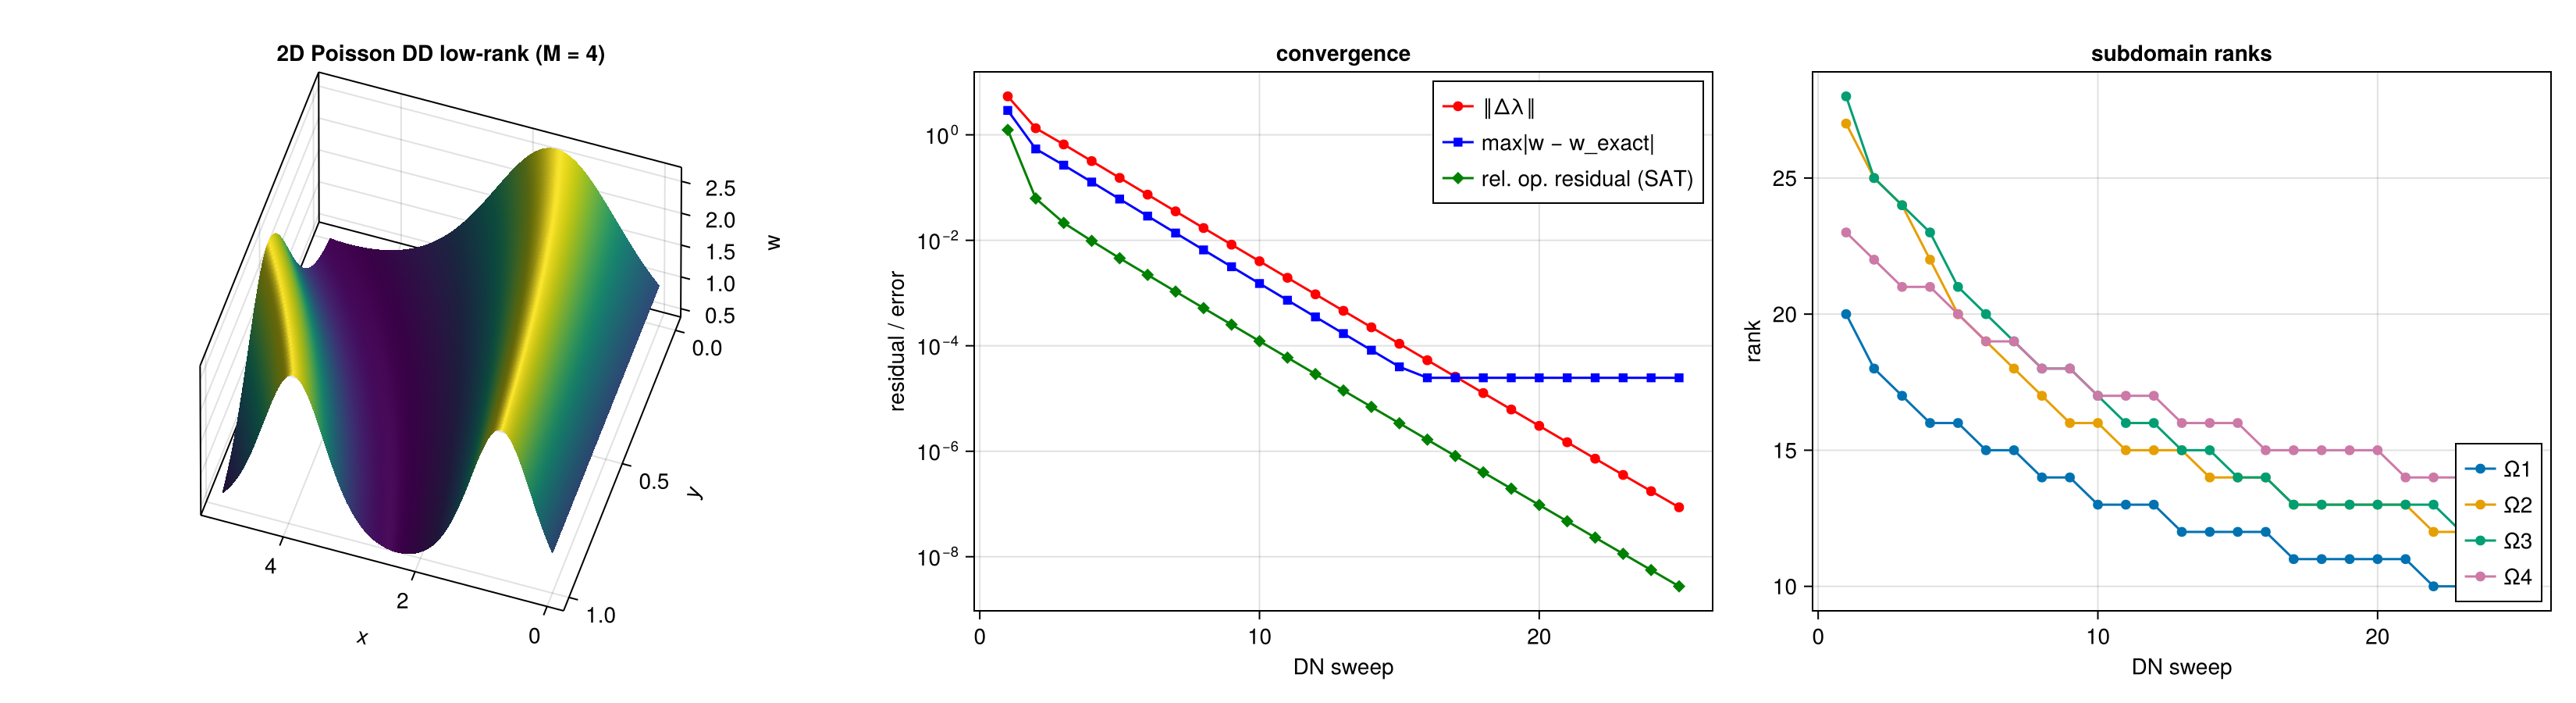
\includegraphics[width=\textwidth]{dn_convergence}
\caption{Representative DN iteration with {\tt eig2d\_lr} ($M=4$, $n_x=n_y=80$,
$p=6$).  Left: assembled low-rank solution.  Middle: interface increment
$\|\Delta\lambda\|$, maximum error, and relative SBP--SAT operator residual vs.\
sweep.  Right: per-subdomain rank vs.\ sweep.\label{fig:dn}}
\end{center}
\end{figure}

\subsection{Order of accuracy}
To isolate the discretization error we use the exact subdomain solver
{\tt eig2d} with a tight DN tolerance ($\TOL_{\rm DD}=10^{-11}$) and refine
$n_x=n_y=N$.  \Cref{tab:refine} reports the maximum error and the observed
convergence rate.  The diagonal-norm SBP--SAT discretization converges at the
expected global rate $p/2+1$: order $\approx 3$ for $p=4$ and $\approx 4$ for
$p=6$.

\begin{table}[htb]
\caption{Grid refinement with the exact solver {\tt eig2d} ($M=4$,
$\TOL_{\rm DD}=10^{-11}$).  Observed rate $=\log(e_{N/2}/e_N)/\log 2$.
\label{tab:refine}}
\begin{center}
\begin{tabular}{r r c r c}
\toprule
 & \multicolumn{2}{c}{$p=4$} & \multicolumn{2}{c}{$p=6$} \\
\cmidrule(lr){2-3}\cmidrule(lr){4-5}
$N$ & max error & rate & max error & rate \\
\midrule
$20$  & $3.23\times10^{-3}$ & ---  & $8.53\times10^{-3}$ & ---  \\
$40$  & $3.36\times10^{-4}$ & $3.14$ & $4.56\times10^{-4}$ & $4.07$ \\
$80$  & $3.75\times10^{-5}$ & $3.11$ & $2.47\times10^{-5}$ & $4.13$ \\
$160$ & $4.40\times10^{-6}$ & $3.06$ & $1.42\times10^{-6}$ & $4.12$ \\
\bottomrule
\end{tabular}
\end{center}
\end{table}

\subsection{Comparison of the three subdomain solvers}
\Cref{tab:solvers} compares the three solvers on a fixed problem
($n_x=n_y=80$, $p=6$, $\TOL_{\rm DD}=10^{-7}$) with the final truncation
tolerance matched at $\epsilon_{\rm trunc}=10^{-10}$ so the reported ranks are
comparable.  All three reach the discretization error
$\approx 2.5\times10^{-5}$ in the same number of DN sweeps ($25$): the outer DN
iteration count is set by the interface coupling and is essentially independent
of which subdomain solver is used.  The low-rank solver {\tt eig2d\_lr} attains
this accuracy while operating entirely on the factors --- it never forms a dense
$n_x\times n_y$ subdomain matrix --- and at a rank comparable to (here below) the
truncated dense solvers, because its core truncation \cref{eq:gfun} compresses
the diagonalized solution directly.

\begin{table}[htb]
\caption{Solver comparison ($M=4$, $n_x=n_y=80$, $p=6$, $\TOL_{\rm DD}=10^{-7}$,
$\epsilon_{\rm trunc}=10^{-10}$).  ``max rank''/``mean rank'' are over the four
subdomains at convergence.\label{tab:solvers}}
\begin{center}
\begin{tabular}{l c c c c}
\toprule
solver & DN sweeps & max error & max rank & mean rank \\
\midrule
{\tt eig2d} (direct)    & $25$ & $2.470\times10^{-5}$ & $20$ & $17.0$ \\
{\tt cg2d} (iterative)  & $25$ & $2.469\times10^{-5}$ & $20$ & $17.5$ \\
{\tt eig2d\_lr}         & $25$ & $2.470\times10^{-5}$ & $14$ & $11.8$ \\
\bottomrule
\end{tabular}
\end{center}
\end{table}

\subsection{Truncation tolerance, rank, and robustness}
\label{sec:exp-rank}
For {\tt eig2d\_lr} the truncation tolerance $\epsilon_{\rm trunc}$ is the
rank/accuracy knob.  \Cref{tab:rank} and \cref{fig:rank} show, for the fixed
problem of \cref{tab:solvers}, that decreasing $\epsilon_{\rm trunc}$ raises the
converged rank while the error saturates at the discretization floor: once
$\epsilon_{\rm trunc}\lesssim 10^{-6}$ the error is already
$\approx 2.5\times10^{-5}$, attained at mean rank $7.5$ (versus $17$ at
$\epsilon_{\rm trunc}=10^{-12}$).  The per-sweep rank (\cref{fig:rank}) settles
to a level set by the tolerance.

\begin{table}[htb]
\caption{Effect of the truncation tolerance on {\tt eig2d\_lr} ($M=4$,
$n_x=n_y=80$, $p=6$, $\TOL_{\rm DD}=10^{-7}$).\label{tab:rank}}
\begin{center}
\begin{tabular}{c c c c c}
\toprule
$\epsilon_{\rm trunc}$ & DN sweeps & max error & max rank & mean rank \\
\midrule
$10^{-6}$  & $26$ & $2.477\times10^{-5}$ & $9$  & $7.5$  \\
$10^{-8}$  & $25$ & $2.471\times10^{-5}$ & $11$ & $9.5$  \\
$10^{-10}$ & $25$ & $2.470\times10^{-5}$ & $14$ & $11.8$ \\
$10^{-12}$ & $25$ & $2.470\times10^{-5}$ & $20$ & $17.0$ \\
\bottomrule
\end{tabular}
\end{center}
\end{table}

\begin{figure}[htb]
\begin{center}
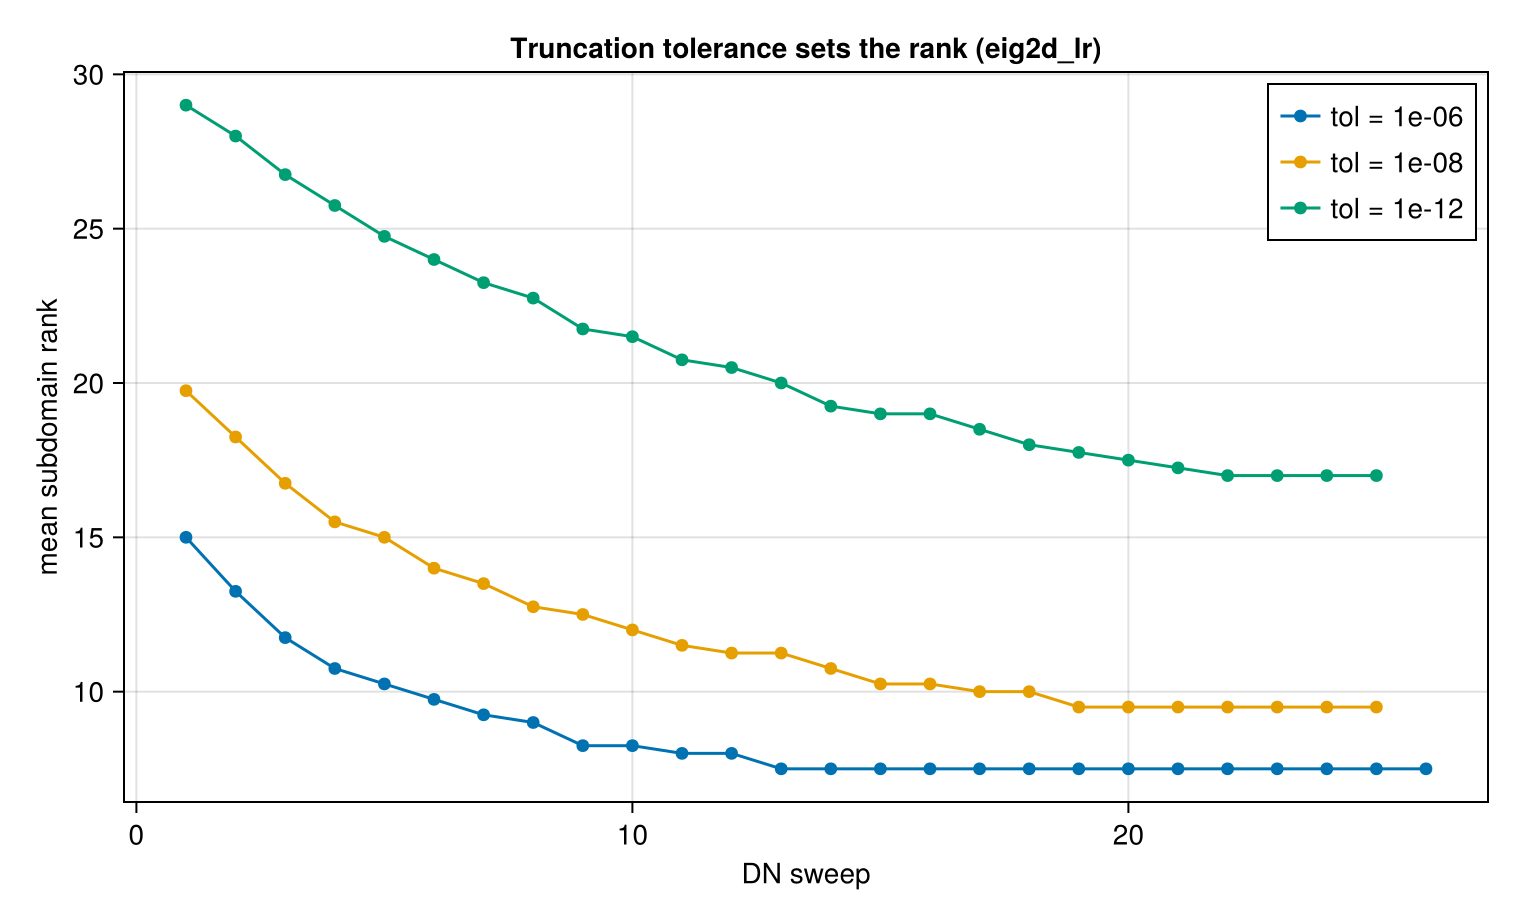
\includegraphics[width=0.6\textwidth]{rank_vs_tol}
\caption{Mean subdomain rank vs.\ DN sweep for {\tt eig2d\_lr} at three
truncation tolerances ($M=4$, $n_x=n_y=80$, $p=6$).  A tighter tolerance settles
to a higher rank.\label{fig:rank}}
\end{center}
\end{figure}

Finally, \cref{fig:tolstudy} reports the converged error as the DN tolerance
$\TOL_{\rm DD}$ is varied over $10^{-3}$ to $10^{-9}$ on a coarser grid
($n_x=25$, $n_y=101$).  The error is essentially flat at the discretization
floor ($\approx 3.4\times10^{-3}$) across the whole range, and the low-rank
solver {\tt eig2d\_lr} tracks the exact solver {\tt eig2d} for every tolerance;
only {\tt cg2d} with a loose solver tolerance ($10^{-7}$) shows minor noise.
This is the robustness one wants: the achievable accuracy is governed by the
discretization, not by the choice of DN tolerance or subdomain solver, provided
the latter is not starved of accuracy.

\begin{figure}[htb]
\begin{center}
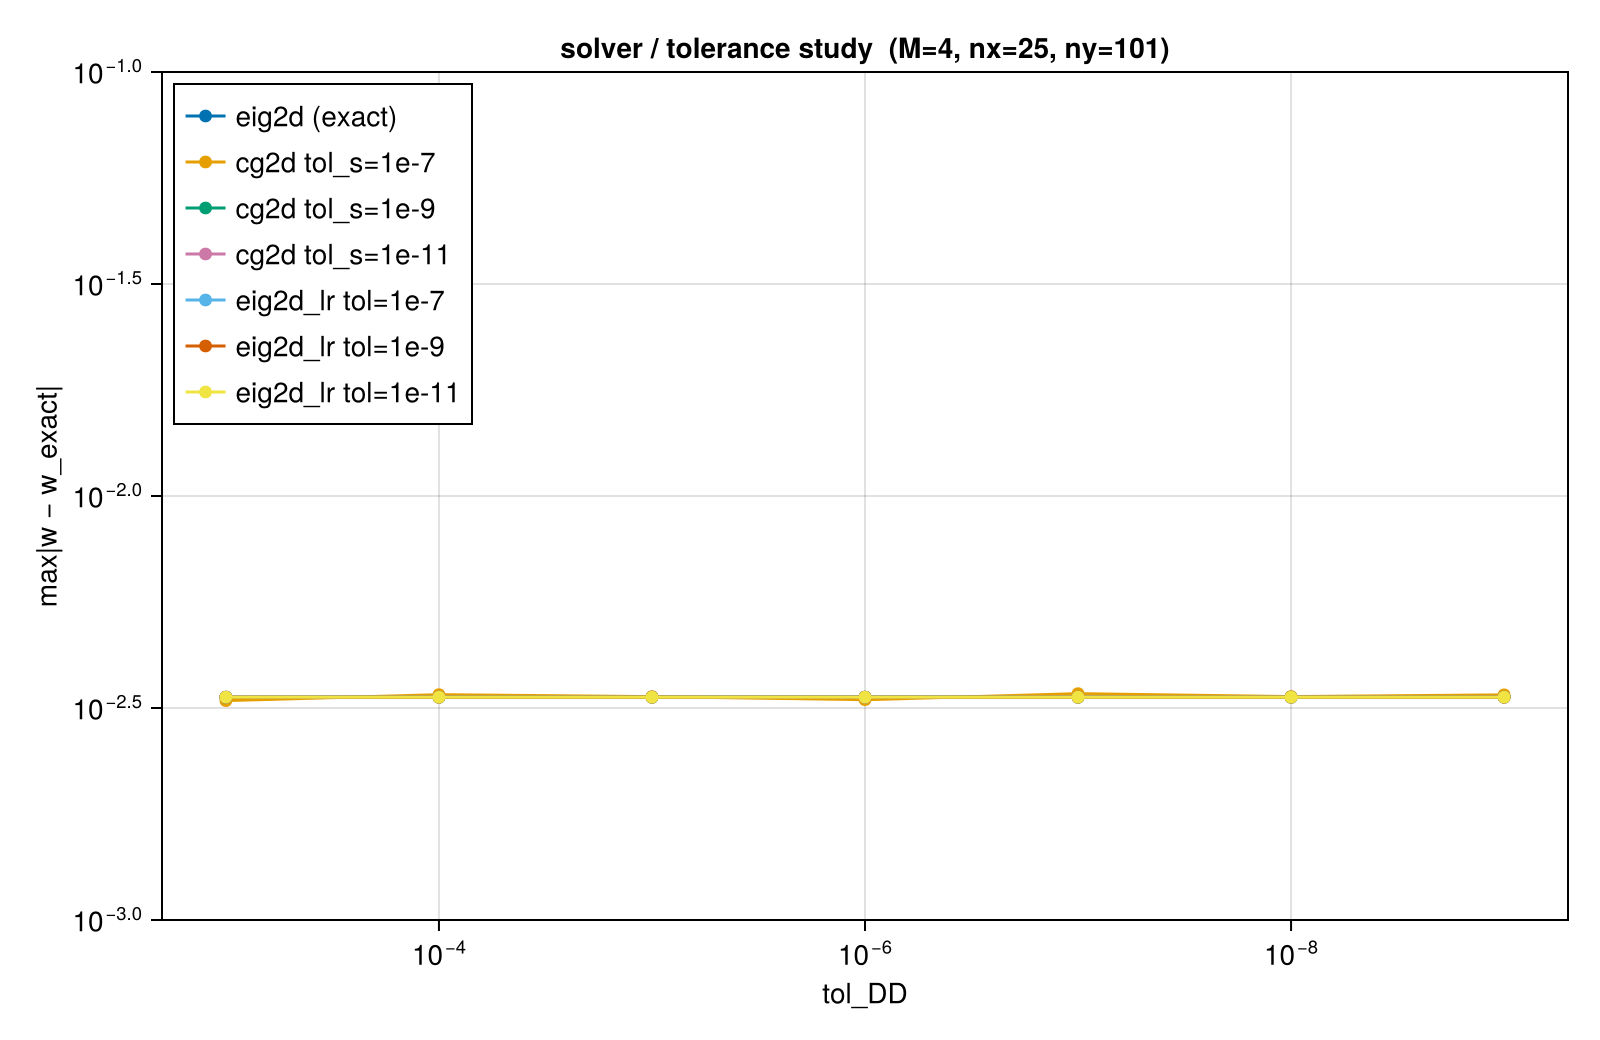
\includegraphics[width=0.62\textwidth]{tolerance_study}
\caption{Converged maximum error vs.\ DN tolerance $\TOL_{\rm DD}$ for the three
solvers ($M=4$, $n_x=25$, $n_y=101$); the $x$-axis decreases to the right.  All
curves sit at the discretization floor.\label{fig:tolstudy}}
\end{center}
\end{figure}

\subsection{The tolerance schedule: choosing $\theta$ and rank growth}
\label{sec:exp-schedule}
We now study the adaptive schedule \cref{eq:sched} for {\tt eig2d\_lr} on the
fixed problem of \cref{tab:solvers} ($M=4$, $n_x=n_y=80$, $p=6$,
$\TOL_{\rm DD}=10^{-7}$), with floor $\epsilon_{\min}=10^{-10}$ unless stated
otherwise.

\paragraph{Choosing the constant $\theta$.}  \Cref{tab:theta} and the left panel
of \cref{fig:sched} sweep the schedule constant $\theta$.  There is a sharp
threshold near $\theta^\ast\approx0.05$.  For $\theta\gtrsim0.07$ the iteration
locks onto the spurious low-rank fixed point described in \cref{sec:schedule}:
the interface increment $\rho=\|\Delta\lambda\|$ becomes small, the schedule keeps
$\epsilon_k=\theta\rho_{k-1}$ loose, and the error stalls two to four orders of
magnitude above the discretization floor (e.g.\ $2.2\times10^{-2}$ at
$\theta=0.10$) at rank $5$--$6$.  For $\theta\le0.03$ the schedule is robust: it
converges to the discretization error $2.5\times10^{-5}$ in $24$--$34$ sweeps.
The case $\theta=0.05$ is borderline --- it reaches the discretization error but
does not drive $\rho$ below $\TOL_{\rm DD}$ within the sweep budget.  Within the
robust range, a smaller $\theta$ converges in slightly fewer sweeps at a
marginally higher rank, so we recommend $\theta\approx0.01$--$0.03$.

\begin{table}[htb]
\caption{Robustness of the schedule \cref{eq:sched} versus the constant $\theta$
($M=4$, $n_x=n_y=80$, $p=6$, $\TOL_{\rm DD}=10^{-7}$, $\epsilon_{\min}=10^{-10}$,
budget $400$ sweeps).  ``peak rank'' is the maximum rank over all sweeps.
\label{tab:theta}}
\begin{center}
\begin{tabular}{c c c c c c}
\toprule
$\theta$ & converged & DN sweeps & max error & final rank & peak rank \\
\midrule
$0.10$ & no  & $400$ & $2.16\times10^{-2}$ & $5$  & $6$  \\
$0.07$ & no  & $400$ & $1.86\times10^{-2}$ & $6$  & $6$  \\
$0.05$ & no  & $400$ & $2.48\times10^{-5}$ & $9$  & $10$ \\
$0.03$ & yes & $34$  & $2.47\times10^{-5}$ & $12$ & $12$ \\
$0.02$ & yes & $28$  & $2.47\times10^{-5}$ & $12$ & $12$ \\
$0.01$ & yes & $24$  & $2.47\times10^{-5}$ & $13$ & $13$ \\
\bottomrule
\end{tabular}
\end{center}
\end{table}

\paragraph{The floor $\epsilon_{\min}$.}  At a robust $\theta=0.02$ the schedule
is insensitive to the floor: varying $\epsilon_{\min}$ from $10^{-7}$ to
$10^{-12}$ converges in $26$--$28$ sweeps to the discretization error, with the
final rank rising only mildly from $10$ to $12$ as the floor tightens.  The floor
should be taken at or below $\TOL_{\rm DD}$ and is otherwise forgiving; it sets
the final rank rather than whether the method converges.

\paragraph{Rank growth under scheduling.}  The right panel of \cref{fig:sched}
contrasts the per-sweep rank of the robust schedule ($\theta=0.02$) with that of
a fixed tight tolerance ($\epsilon_{\rm trunc}=10^{-10}$), both reaching the same
accuracy.  With scheduling the mean rank grows \emph{near-monotonically} from $1$
to its converged value, and the peak rank equals the final rank ($12$).  With the
fixed tolerance the rank instead starts high --- the first sweeps resolve a poor
interface guess to full tolerance --- peaking at $28$ before decaying to a final
$14$.  Scheduling thus more than halves the peak intermediate rank ($12$ vs.\
$28$) at the same final accuracy and a comparable sweep count, which is precisely
the rank-control behavior sought from a rank-adaptive low-rank method.

\begin{figure}[htb]
\begin{center}
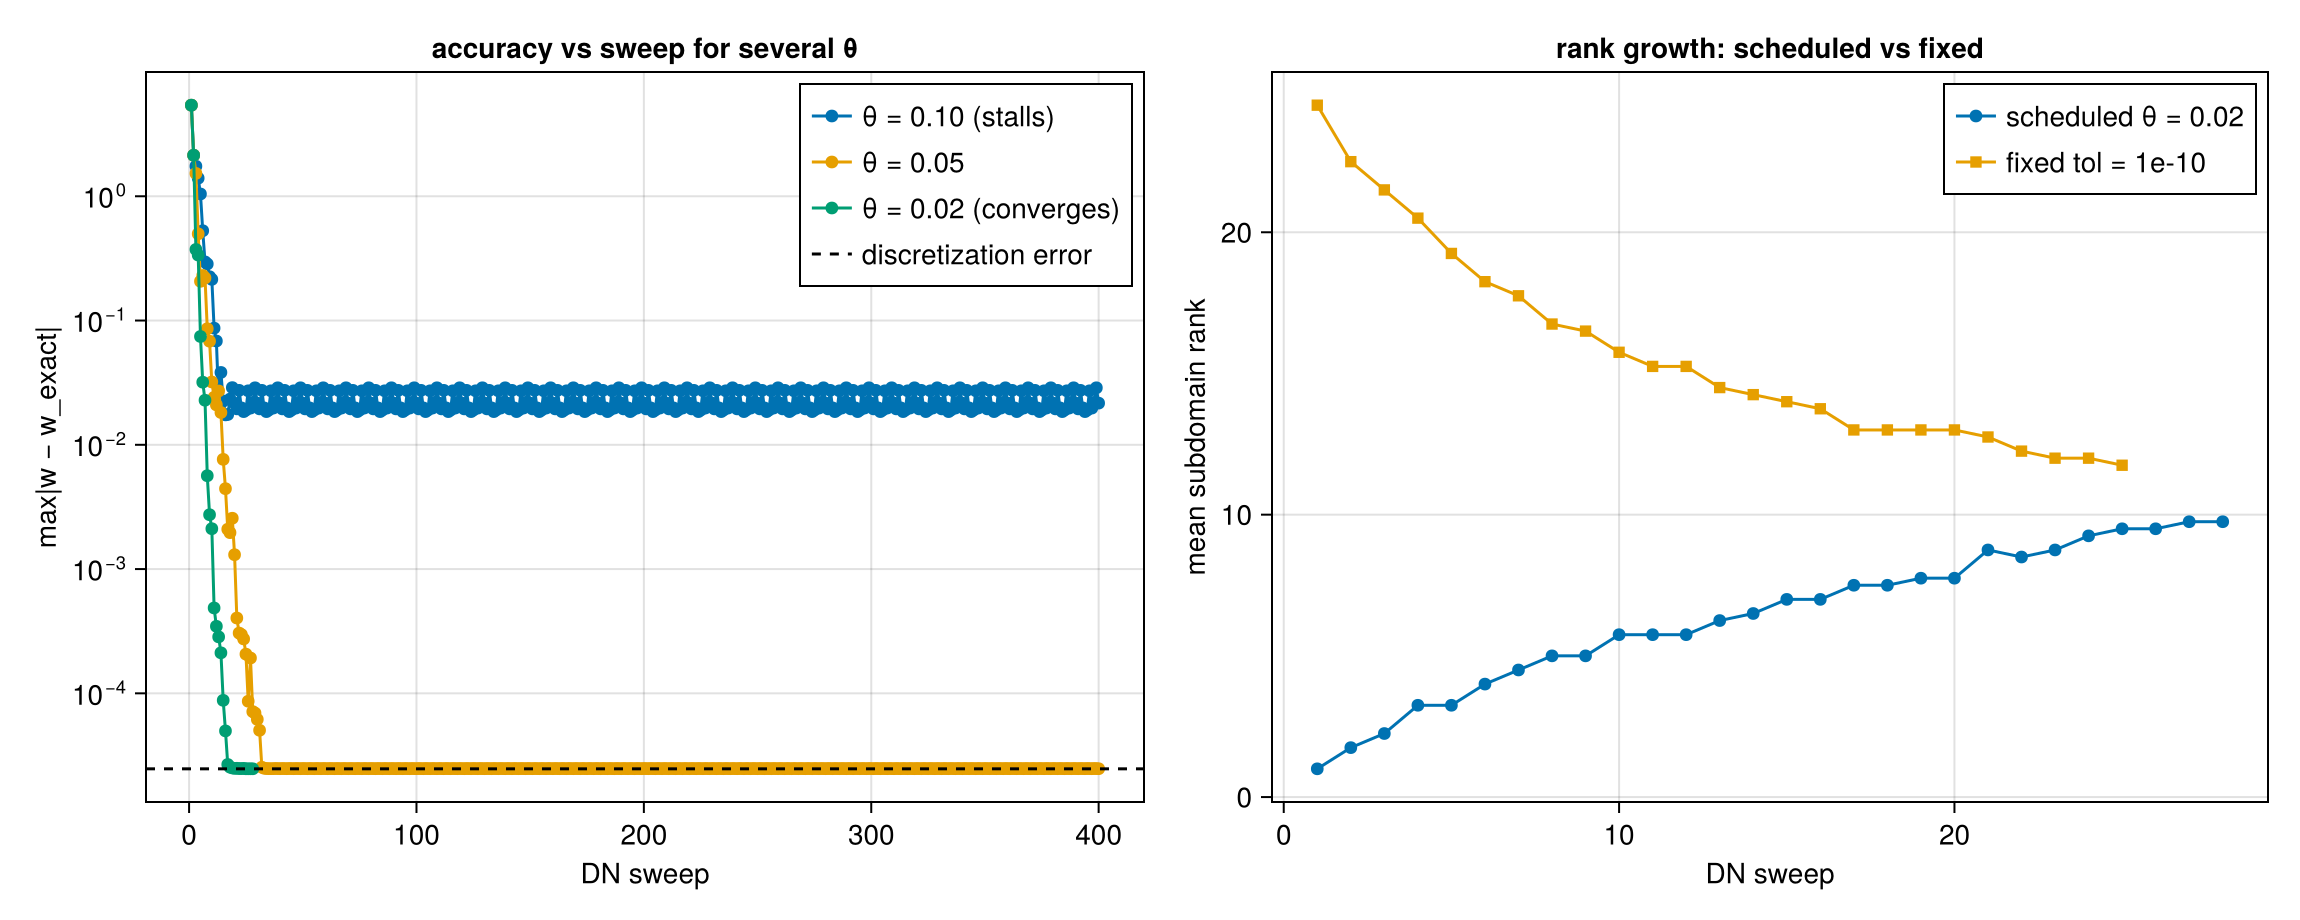
\includegraphics[width=\textwidth]{scheduling}
\caption{Adaptive schedule \cref{eq:sched} for {\tt eig2d\_lr} ($M=4$,
$n_x=n_y=80$, $p=6$).  Left: maximum error vs.\ sweep for several $\theta$; large
$\theta$ stalls above the discretization error (dashed), small $\theta$ converges
to it.  Right: mean subdomain rank vs.\ sweep --- the robust schedule
($\theta=0.02$) grows the rank from $1$ near-monotonically, whereas a fixed tight
tolerance starts high and decays.\label{fig:sched}}
\end{center}
\end{figure}

\paragraph{A more robust schedule: driving by the operator residual.}  The
fragility above is a property of the \emph{driving residual}, not of scheduling
itself.  Replacing $\|\Delta\lambda\|$ by the operator residual $R$ of
\cref{eq:opres} in \cref{eq:sched-source} --- a true residual that shrinks only
with genuine progress --- removes the spurious-fixed-point trap.
\Cref{tab:sched-src} repeats the $\theta$ sweep for both sources at $M=4$: the
$R$-driven schedule converges for every $\theta\le0.2$ (only $\theta=0.5$ stalls),
a robust range roughly an order of magnitude wider than the $\|\Delta\lambda\|$
source, and it does so in $23$--$30$ sweeps at the same rank.  The left panel of
\cref{fig:sched-src} makes the mechanism visible at $\theta=0.10$: the
$\|\Delta\lambda\|$ schedule freezes at error $\approx2\times10^{-2}$, while the
$R$ schedule drives the error to the discretization floor in about $20$ sweeps.
The right panel confirms that the $R$-driven schedule retains the desired
near-monotone rank growth (peak rank $13$ versus $28$ for the fixed tolerance).

\begin{table}[htb]
\caption{Schedule source at $M=4$ ($n_x=n_y=80$, $p=6$, $\TOL_{\rm DD}=10^{-7}$,
$\epsilon_{\min}=10^{-10}$, budget $400$ sweeps): interface increment
$\|\Delta\lambda\|$ versus operator residual $R$.\label{tab:sched-src}}
\begin{center}
\begin{tabular}{c c c c c c}
\toprule
 & \multicolumn{2}{c}{$\rho=\|\Delta\lambda\|$} & \multicolumn{3}{c}{$\rho=R$ (operator residual)} \\
\cmidrule(lr){2-3}\cmidrule(lr){4-6}
$\theta$ & converged & max error & converged & DN sweeps & max error \\
\midrule
$0.50$ & no  & $1.2\times10^{0}$  & no  & ---  & $2.4\times10^{-1}$ \\
$0.20$ & no  & $2.4\times10^{-1}$ & yes & $30$ & $2.47\times10^{-5}$ \\
$0.10$ & no  & $2.2\times10^{-2}$ & yes & $25$ & $2.47\times10^{-5}$ \\
$0.05$ & no  & $2.5\times10^{-5}$ & yes & $24$ & $2.47\times10^{-5}$ \\
$0.02$ & yes & $2.47\times10^{-5}$ & yes & $23$ & $2.47\times10^{-5}$ \\
$0.01$ & yes & $2.47\times10^{-5}$ & yes & $24$ & $2.47\times10^{-5}$ \\
\bottomrule
\end{tabular}
\end{center}
\end{table}

\begin{figure}[htb]
\begin{center}
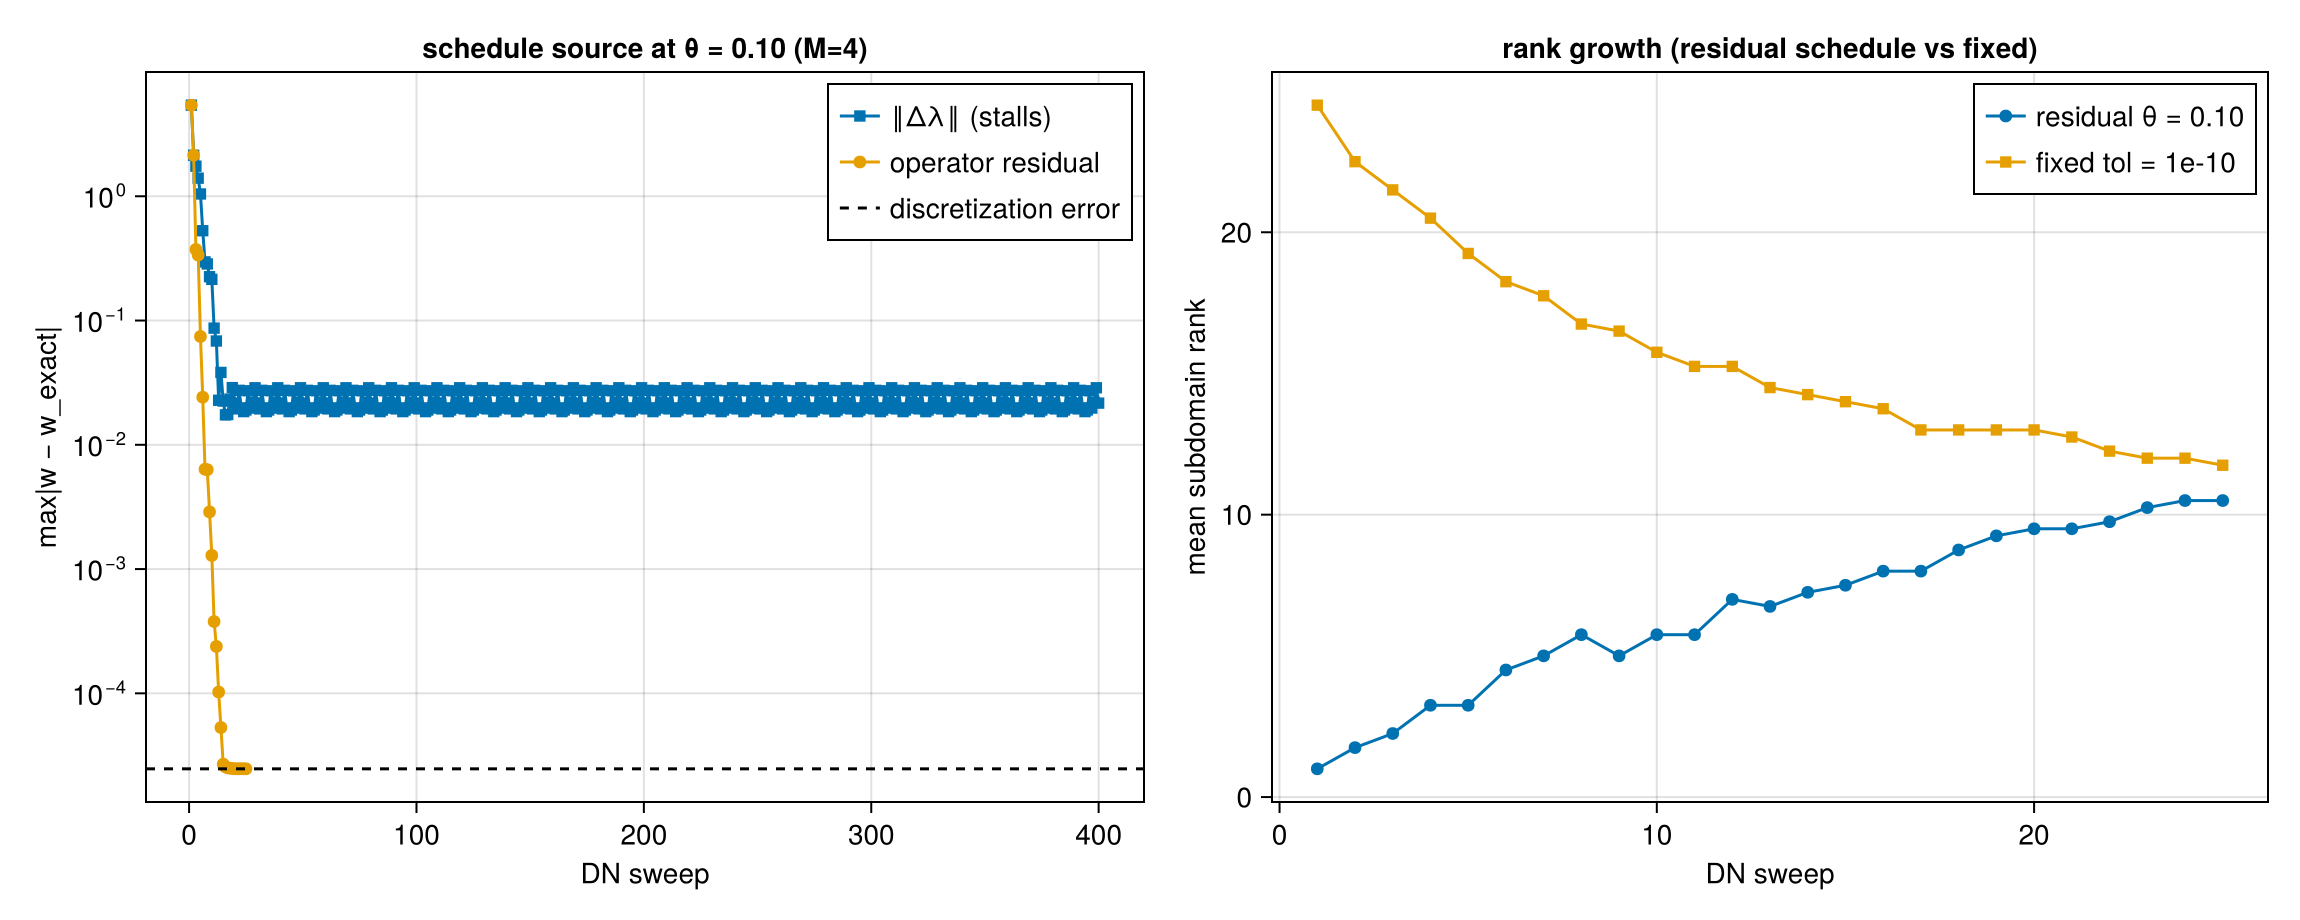
\includegraphics[width=\textwidth]{scheduling_residual}
\caption{Schedule driven by the operator residual $R$ versus the interface
increment $\|\Delta\lambda\|$ ($M=4$, $n_x=n_y=80$, $p=6$).  Left: maximum error
vs.\ sweep at $\theta=0.10$ --- the $\|\Delta\lambda\|$ schedule stalls, the $R$
schedule converges to the discretization floor (dashed).  Right: the $R$-driven
schedule grows the rank near-monotonically from $1$, like the robust
$\|\Delta\lambda\|$ case, far below the fixed-tolerance peak.\label{fig:sched-src}}
\end{center}
\end{figure}

The improvement is largest at $M=4$; the threshold still shrinks as the number of
subdomains grows, but the $R$-driven schedule remains uniformly more forgiving.
Measuring the largest converging $\theta$ on the $n_x=n_y=48$ problem of
\cref{sec:exp-sub}, the $\|\Delta\lambda\|$ source gives $\theta^\ast\approx
0.02,\,0.01,\,0.005$ at $M=4,8,16$, while the $R$ source gives $\theta^\ast\approx
0.2,\,0.02,\,0.01$ --- a factor of $\sim2$ at the larger $M$ and $\sim10$ at
$M=4$.  We therefore use the operator-residual source by default when scheduling.

\section{Computational cost and scaling}
\label{sec:cost}
We close with two scaling studies comparing the dense direct solver {\tt eig2d}
with the scheduled low-rank solver {\tt eig2d\_lr}: wall-clock time as the grid
is refined, and the DN iteration count as the number of subdomains grows.  The
timings are wall-clock seconds on a single workstation and are indicative; the
robust conclusions are the scaling exponents and the crossover, not the absolute
times.

\subsection{Timing versus grid size}
\label{sec:exp-timing}
\Cref{tab:timing} and \cref{fig:timing} report the time to solve to
$\TOL_{\rm DD}=10^{-7}$ with $M=4$, $p=6$, as the per-subdomain grid is refined
($n_x=n_y=N$).  Both solvers share the same one-time $O(N^3)$ symmetric
eigendecomposition of the $1$D operators; they differ in the per-sweep work,
which is a pair of dense $O(N^3)$ matrix products for {\tt eig2d} (forming
$Q_1^{\!\top}BQ_2$ and $Q_1YQ_2^{\!\top}$) versus the $O(N^2 r)$ factor rotations
\cref{eq:eig2dlr} plus a Cross-DEIM solve for {\tt eig2d\_lr}.  As both reach the
discretization error in the \emph{same} number of sweeps (\cref{tab:solvers}),
the timing reflects this per-sweep difference.  At small $N$ the Cross-DEIM
overhead makes {\tt eig2d\_lr} several times slower, but it scales with a smaller
exponent (empirically $\approx N^{1.8}$ versus $\approx N^{2.4}$ for
{\tt eig2d}); the two cross over near $N\approx320$, and at $N=640$ the low-rank
solver is $2.1\times$ faster.

\begin{table}[htb]
\caption{Wall-clock solve time vs.\ grid size $N=n_x=n_y$ ($M=4$, $p=6$,
$\TOL_{\rm DD}=10^{-7}$; {\tt eig2d\_lr} scheduled with $\theta=0.02$).  Times are
the minimum of two runs.\label{tab:timing}}
\begin{center}
\begin{tabular}{r r r c}
\toprule
$N$ & {\tt eig2d} [s] & {\tt eig2d\_lr} [s] & speedup ({\tt eig2d}/{\tt eig2d\_lr}) \\
\midrule
$40$  & $0.034$  & $0.234$ & $0.14$ \\
$80$  & $0.116$  & $0.448$ & $0.26$ \\
$160$ & $0.500$  & $0.842$ & $0.59$ \\
$320$ & $2.464$  & $1.941$ & $1.27$ \\
$640$ & $13.379$ & $6.292$ & $2.13$ \\
\bottomrule
\end{tabular}
\end{center}
\end{table}

\begin{figure}[htb]
\begin{center}
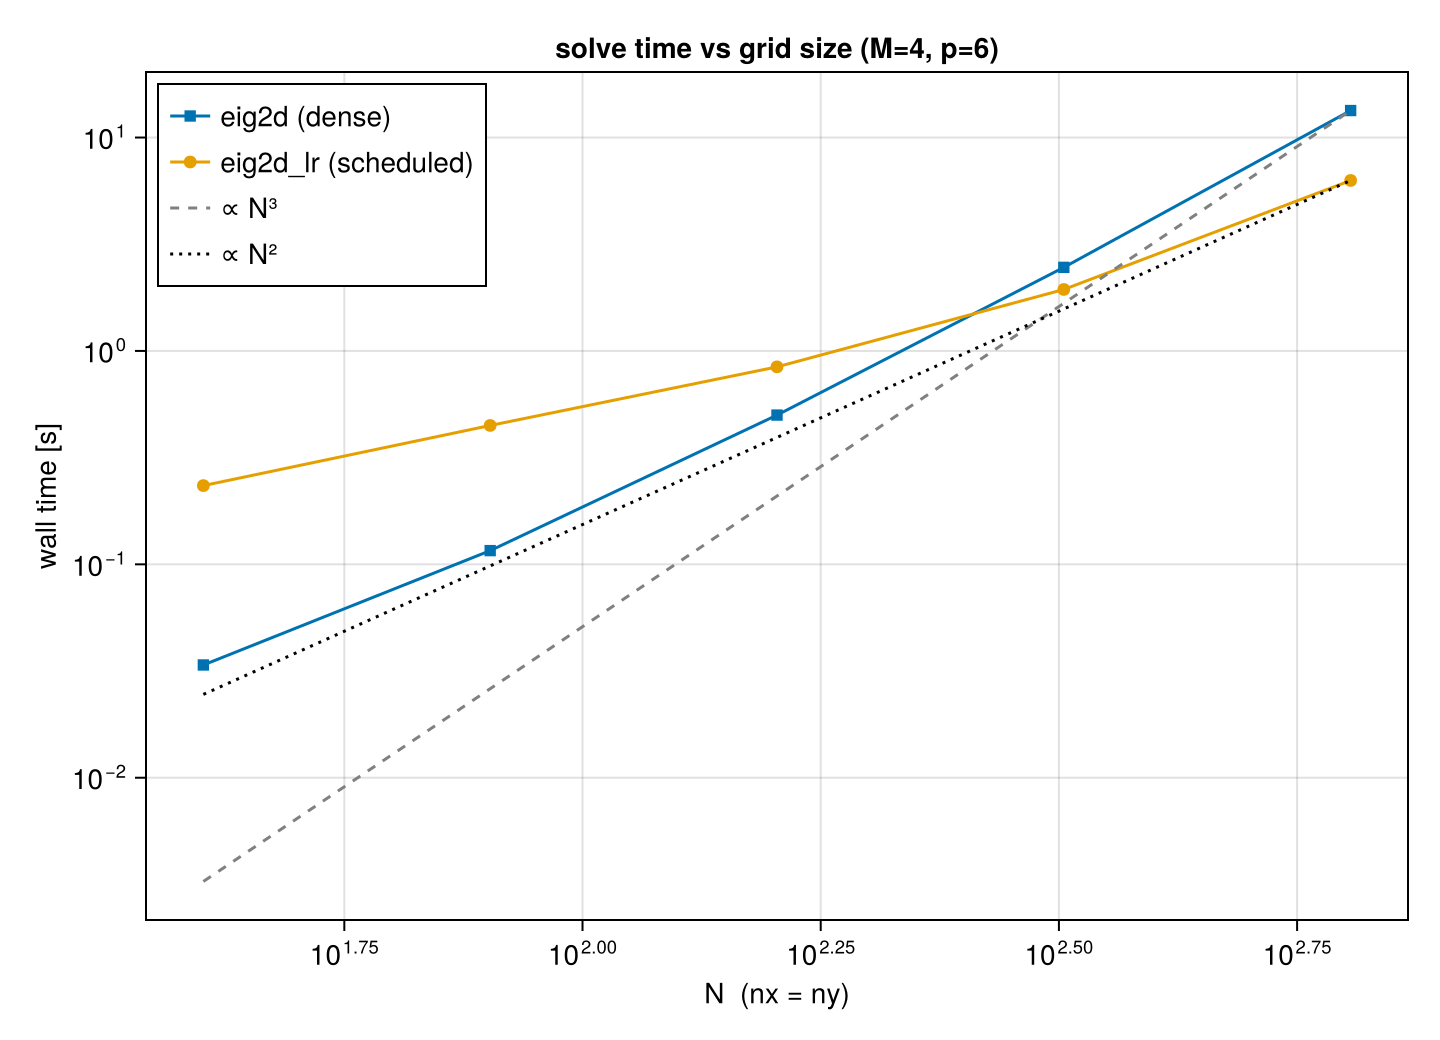
\includegraphics[width=0.6\textwidth]{timing}
\caption{Wall-clock solve time vs.\ grid size $N$ ($M=4$, $p=6$), log--log.  The
dense {\tt eig2d} grows like $\approx N^{2.4}$ (dashed $\propto N^3$ reference),
the scheduled {\tt eig2d\_lr} like $\approx N^{1.8}$ (dotted $\propto N^2$
reference); they cross near $N\approx320$.\label{fig:timing}}
\end{center}
\end{figure}

\subsection{Iteration count versus the number of subdomains}
\label{sec:exp-sub}
\Cref{tab:sub} and \cref{fig:sub} fix the per-subdomain grid ($n_x=n_y=48$,
$p=6$) and vary the number of strips $M$.  Here {\tt eig2d\_lr} uses a fixed tight
tolerance ($\epsilon_{\rm trunc}=10^{-10}$) so that both solvers converge to
$\TOL_{\rm DD}=10^{-7}$.  The headline observation answers the comparison
question directly: \emph{the DN sweep count is identical for {\tt eig2d} and
{\tt eig2d\_lr}} at every $M$ --- the outer iteration is governed by the interface
coupling, not by how the subdomain solve is represented --- and {\tt eig2d\_lr}
simply does it at a lower rank.  The one-level Dirichlet--Neumann iteration is not
scalable in $M$: the sweep count is nearly flat for small $M$ but grows roughly
like $M^2$ for larger $M$ (from $25$ at $M=4$ to $457$ at $M=32$), as expected
without a coarse-grid correction.

\begin{table}[htb]
\caption{DN sweeps to reach $\TOL_{\rm DD}=10^{-7}$ vs.\ number of subdomains $M$
($n_x=n_y=48$, $p=6$).  {\tt eig2d\_lr} uses a fixed $\epsilon_{\rm trunc}=10^{-10}$;
``rank'' is the converged maximum subdomain rank.\label{tab:sub}}
\begin{center}
\begin{tabular}{r c c c c}
\toprule
 & \multicolumn{2}{c}{\tt eig2d} & \multicolumn{2}{c}{\tt eig2d\_lr} \\
\cmidrule(lr){2-3}\cmidrule(lr){4-5}
$M$ & DN sweeps & rank & DN sweeps & rank \\
\midrule
$2$  & $26$  & $22$ & $26$  & $20$ \\
$4$  & $25$  & $20$ & $25$  & $16$ \\
$8$  & $35$  & $16$ & $35$  & $13$ \\
$16$ & $123$ & $13$ & $123$ & $10$ \\
$32$ & $457$ & $11$ & $457$ & $8$  \\
\bottomrule
\end{tabular}
\end{center}
\end{table}

\begin{figure}[htb]
\begin{center}
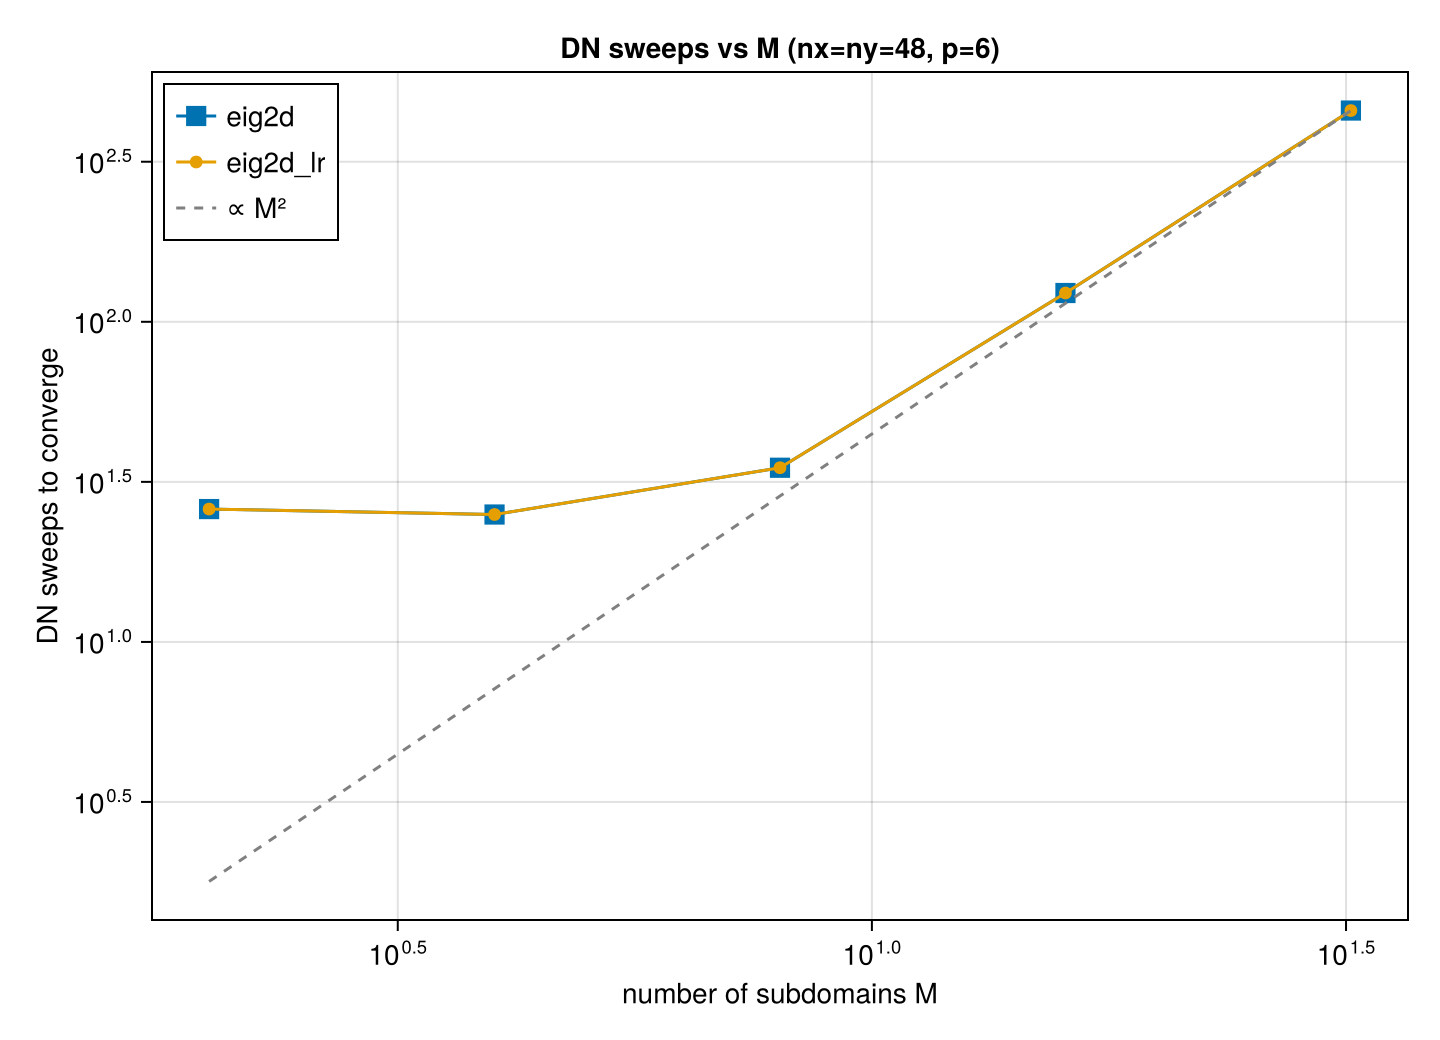
\includegraphics[width=0.6\textwidth]{subdomains}
\caption{DN sweeps to converge vs.\ number of subdomains $M$ ($n_x=n_y=48$,
$p=6$), log--log.  The {\tt eig2d} and {\tt eig2d\_lr} markers coincide; the
growth tracks the $\propto M^2$ reference (dashed) for larger
$M$.\label{fig:sub}}
\end{center}
\end{figure}

There is, however, one genuine difference for the \emph{scheduled} low-rank
solver: the robust range of the schedule constant $\theta$ shrinks as $M$ grows.
With more subdomains the interface increment $\rho=\|\Delta\lambda\|$ per sweep is
smaller relative to the true error, so the schedule of \cref{sec:exp-schedule}
locks onto the spurious fixed point at a smaller $\theta$.  Measuring the largest
tested $\theta$ that still converges, we find $\theta^\ast$ between $0.02$ and
$0.05$ at $M=4$, near $0.01$ at $M=8$, and near $0.005$ at $M=16$ --- roughly
$\theta^\ast\propto 1/M$.  In practice one should therefore scale the schedule
constant down with the number of subdomains (or simply use the fixed-tolerance
{\tt eig2d\_lr}, which has no such restriction and gives the iteration counts of
\cref{tab:sub}).  In the robust range the scheduled solver converges in
essentially the same sweep count as {\tt eig2d} (e.g.\ $37$ vs.\ $35$ at $M=8$,
$129$ vs.\ $123$ at $M=16$).

\section{Three-dimensional Tucker analogue}
\label{sec:3d}
The same construction extends to three dimensions, where the matrix unknown
becomes a 3-tensor $W\in\R^{n_x\times n_y\times n_z}$ stored in \emph{Tucker}
format, $W = \mathcal{G}\times_1 U_1 \times_2 U_2 \times_3 U_3$ (the {\tt Tucker3}
type of {\tt LRDD.jl}).  The domain is split in $x$ into $M$ slabs; the interface
unknowns $\lambda_i$ are now $n_y\times n_z$ planes.  On a slab the SBP--SAT
discretization of $w_{xx}+w_{yy}+w_{zz}=f$ is the symmetric tensor-Sylvester
equation
\begin{equation}
\label{eq:sylv3d}
\AoneS \times_1 \What + \AtwoS \times_2 \What + \AthreeS \times_3 \What = B,
\end{equation}
the direct analogue of \cref{eq:sylvsym}.  This is implemented in
{\tt examples/sbp\_poisson\_bvp\_3d\_lowrank.jl}, with the manufactured solution
$w=e^{\sqrt2\,x}\cos y\cos z + x^3$ (so $f=6x$), Dirichlet $x$/interfaces and
$z$-faces, and Dirichlet-bottom / Neumann-top in $y$.

\paragraph{Solvers.}  Two solvers are implemented, exactly mirroring {\tt cg2d}
and {\tt eig2d}: {\tt cg3d}, a tensor conjugate gradient for
\cref{eq:sylv3d} on $-\mathcal{L}$, and {\tt eig3d}, the direct
eigen-diagonalization in which each entry is divided by
$\lambda^1_i+\lambda^2_j+\lambda^3_k<0$ (the three eigendecompositions are
precomputed).  Both run through a dense bridge: the Tucker right-hand side is
densified, the slab is solved, and the solution is re-compressed to {\tt Tucker3}
by a sequentially-truncated MLSVD (HOSVD) at tolerance $\epsilon_{\rm trunc}$.
A genuine low-rank Tucker solver, {\tt eig3d\_lr} (the analogue of {\tt eig2d\_lr}),
is also available: it eigen-diagonalizes and builds the divided tensor
$Y_{ijk}=\widehat{G}_{ijk}/(\lambda^1_i+\lambda^2_j+\lambda^3_k)$ in Tucker form
with the matrix-free Tucker Cross-DEIM, never forming an $n_x\times n_y\times n_z$
array in the solve; it reproduces {\tt eig3d} to the discretization error at a
comparable Tucker rank.  (The spectrally-truncated {\tt eig3d\_lr\_p} is still a
placeholder.)  Since the flux and interface trace
of the Dirichlet--Neumann coupling are read off the \emph{truncated} Tucker
solution, $\epsilon_{\rm trunc}$ is the rank/accuracy knob and the per-sweep
schedule \cref{eq:sched}--\cref{eq:sched-source} carries over unchanged.

\paragraph{Convergence.}  \Cref{fig:dn3d} shows a representative {\tt eig3d} run
($M=3$, $n_x=16$, $n_y=n_z=24$, $p=4$, $\epsilon_{\rm trunc}=10^{-10}$,
$\TOL_{\rm DD}=10^{-7}$): the interface increment, max error and operator
residual decrease together, the error settles at the discretization floor
$\approx 8.5\times10^{-5}$ in $24$ sweeps, and the per-subdomain Tucker ranks
relax from $\approx 20$ to $\approx 12$.  {\tt cg3d} and {\tt eig3d} agree to the
discretization error, as in 2D.

\begin{figure}[htb]
\begin{center}
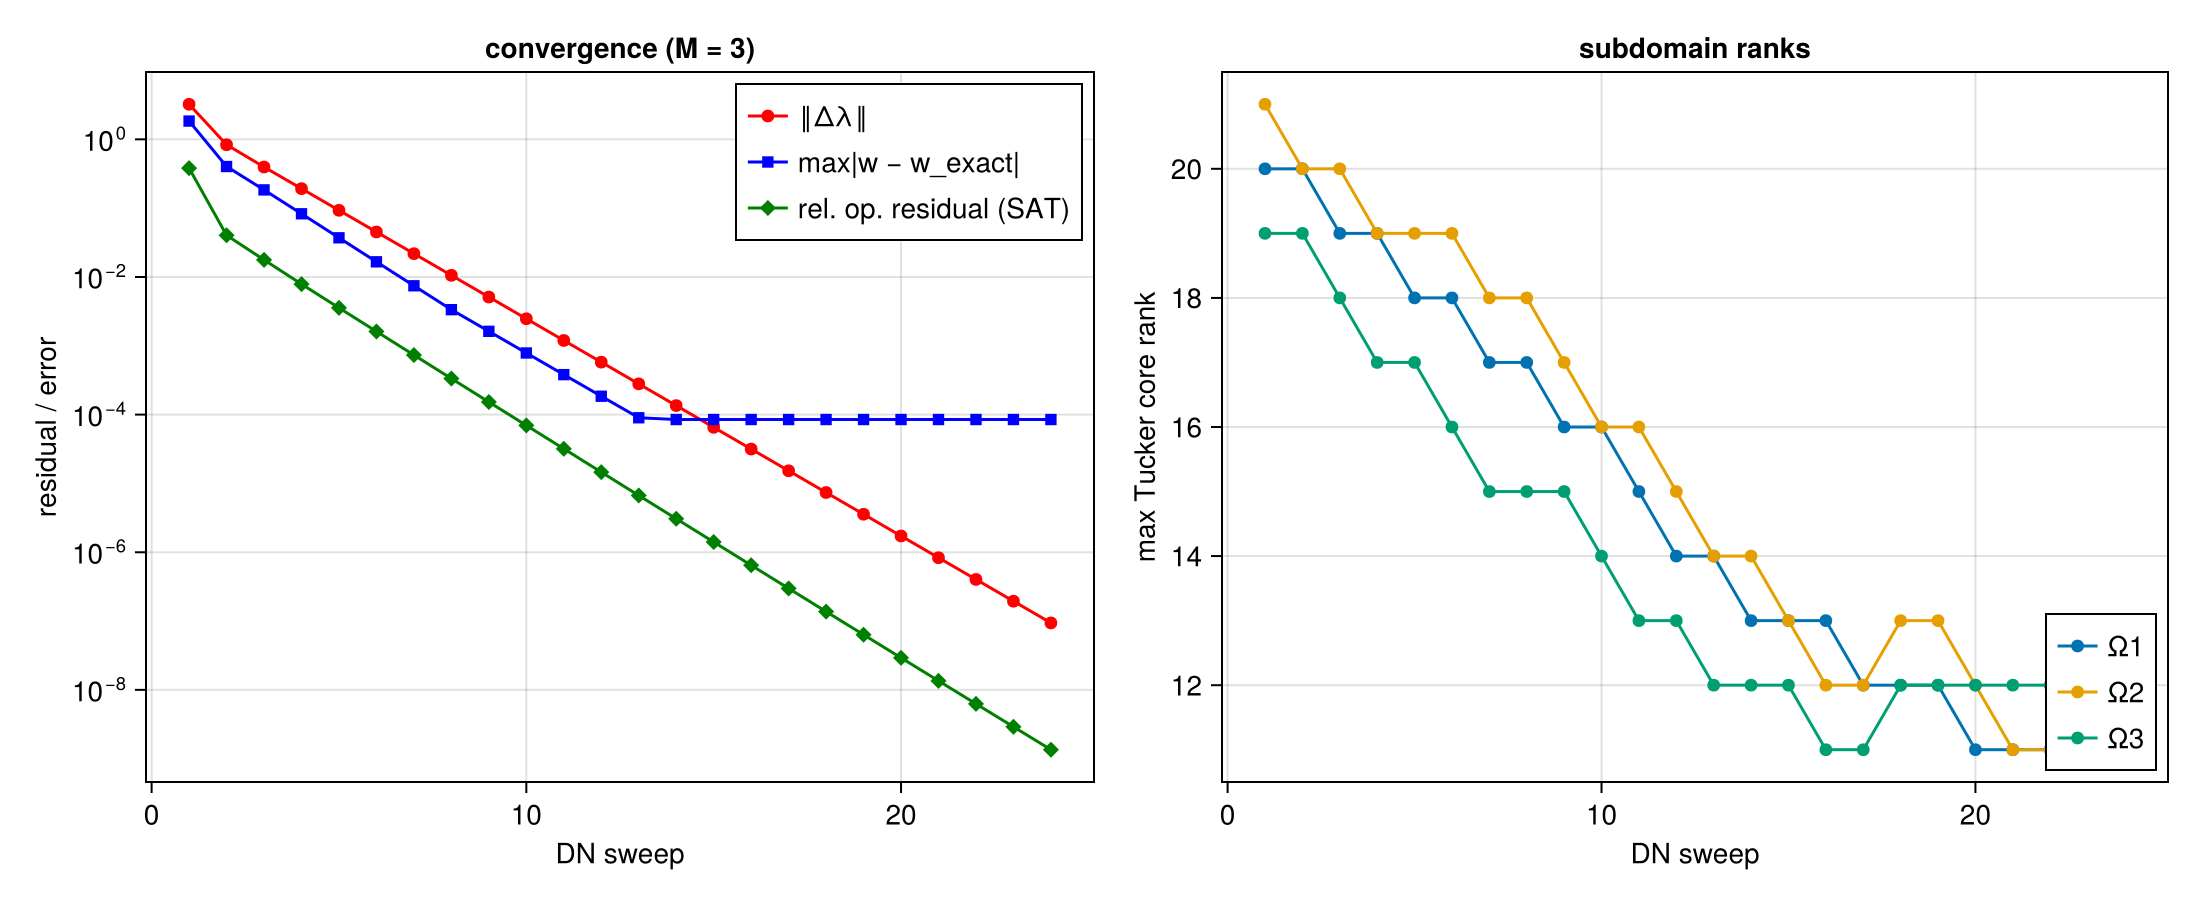
\includegraphics[width=\textwidth]{poisson3d_convergence}
\caption{Representative 3D {\tt eig3d} run ($M=3$, $n_x=16$, $n_y=n_z=24$,
$p=4$).  Left: interface increment $\|\Delta\lambda\|$, max error, and relative
SBP--SAT operator residual vs.\ sweep.  Right: per-subdomain (largest) Tucker
core rank vs.\ sweep.\label{fig:dn3d}}
\end{center}
\end{figure}

\paragraph{Effect of scheduling.}  Adapting $\epsilon_{\rm trunc}$ by the
schedule reproduces the 2D behavior.  \Cref{tab:sched3d} sweeps the constant
$\theta$ for both driving residuals.  The $\|\Delta\lambda\|$ source has a
threshold near $\theta^\ast\approx0.05$: for $\theta\gtrsim0.1$ it fails to drive
$\|\Delta\lambda\|$ below $\TOL_{\rm DD}$, and at $\theta=0.5$ it stalls at a
spurious low-rank fixed point (error $0.24$, rank $2$).  Driving the schedule by
the \emph{operator residual} removes this fragility entirely --- it converges to
the discretization error for every tested $\theta$, including $\theta=0.5$ --- and
the left panel of \cref{fig:sched3d} contrasts the two at $\theta=0.5$.  In its
robust range the schedule delivers near-monotone rank growth (the peak rank
equals the final rank), reaching the discretization-limited solution at a peak
Tucker rank of $8$--$11$ versus $21$ for a fixed tight tolerance, which starts
high and decays (right panel of \cref{fig:sched3d}).  These are the same
conclusions as in 2D, now for the Tucker truncation rank.

\begin{table}[htb]
\caption{3D schedule-source robustness vs.\ $\theta$ ({\tt eig3d}, $M=3$,
$n_x=16$, $n_y=n_z=24$, $p=4$, $\TOL_{\rm DD}=10^{-7}$, $\epsilon_{\min}=10^{-10}$,
budget $400$ sweeps); ``peak rank'' is the maximum core rank over all sweeps and
subdomains.\label{tab:sched3d}}
\begin{center}
\begin{tabular}{c c c c c c}
\toprule
 & \multicolumn{2}{c}{$\rho=\|\Delta\lambda\|$} & \multicolumn{3}{c}{$\rho=R$ (operator residual)} \\
\cmidrule(lr){2-3}\cmidrule(lr){4-6}
$\theta$ & converged & max error & converged & sweeps & peak rank \\
\midrule
$0.50$ & no  & $2.4\times10^{-1}$ & yes & $25$ & $8$  \\
$0.20$ & no  & $6.6\times10^{-5}$ & yes & $24$ & $11$ \\
$0.10$ & no  & $8.6\times10^{-5}$ & yes & $23$ & $11$ \\
$0.05$ & yes & $8.5\times10^{-5}$ & yes & $23$ & $12$ \\
$0.02$ & yes & $8.5\times10^{-5}$ & yes & $23$ & $12$ \\
$0.01$ & yes & $8.5\times10^{-5}$ & yes & $23$ & $12$ \\
\bottomrule
\end{tabular}
\end{center}
\end{table}

\begin{figure}[htb]
\begin{center}
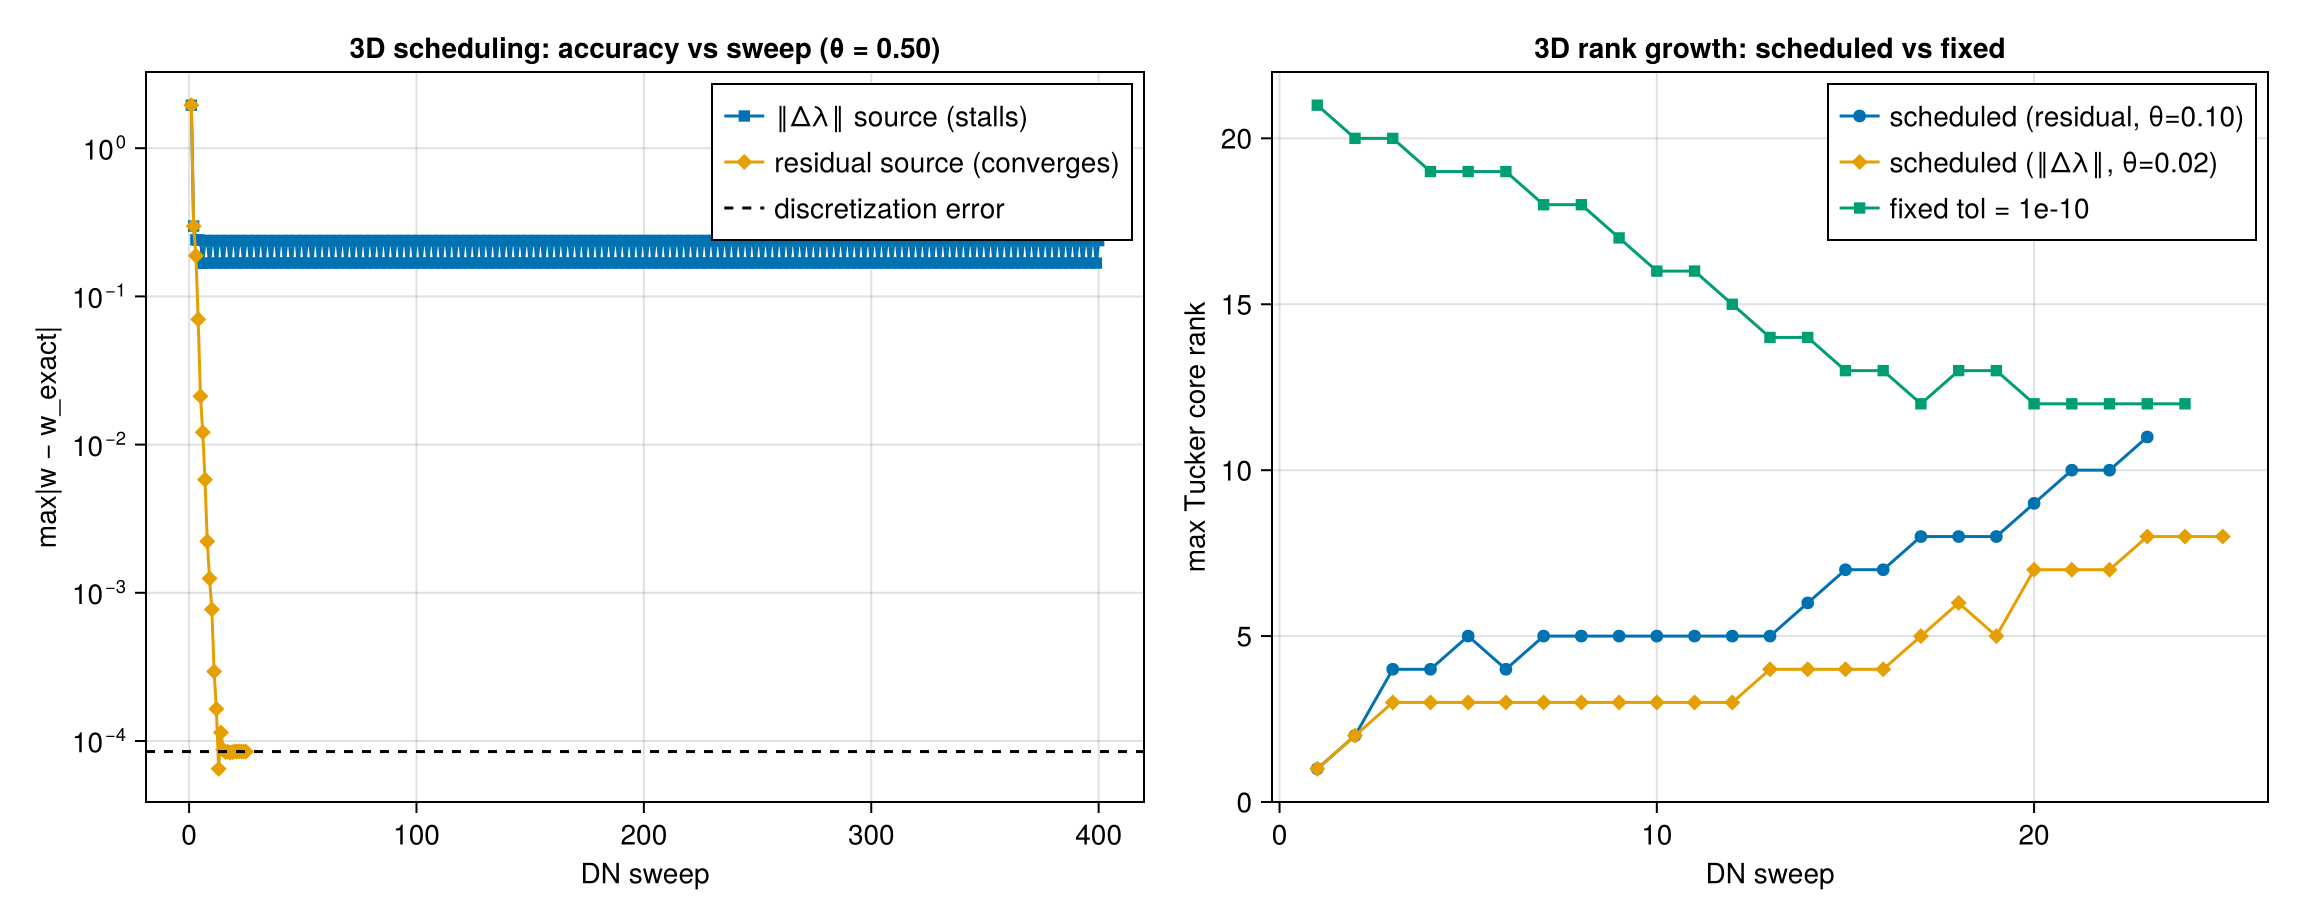
\includegraphics[width=\textwidth]{poisson3d_scheduling}
\caption{3D scheduling ({\tt eig3d}, $M=3$, $n_x=16$, $n_y=n_z=24$).  Left:
max error vs.\ sweep at $\theta=0.5$ --- the $\|\Delta\lambda\|$ source stalls,
the operator-residual source converges to the discretization floor (dashed).
Right: max Tucker core rank vs.\ sweep --- the scheduled runs grow the rank
near-monotonically from $1$, far below the fixed-tolerance peak that starts high
and decays.\label{fig:sched3d}}
\end{center}
\end{figure}

The figures and table are produced by
{\tt examples/experiments/poisson3d\_scheduling.jl}.

\paragraph{Cost at large grids.}  Both 3D solvers share the same dense
right-hand-side bridge --- the boundary injections are full $n_y\times n_z$ (etc.)
interface planes, so the RHS is assembled and compressed densely --- but
{\tt eig3d\_lr} replaces the dense eigen-diagonalization solve with the
matrix-free Tucker Cross-DEIM, which scales better in the grid size.
\Cref{tab:timing3d} times the full Dirichlet--Neumann solution ($M=2$, $p=4$,
$\TOL_{\rm DD}=10^{-7}$) as $N=n_x=n_y=n_z$ grows; all cases converge in $24$
sweeps to the discretization error.  The two solvers cross over near $N\approx150$,
and at the requested $N=300$ (a $300^3$ grid, $54$M unknowns over the two slabs)
{\tt eig3d\_lr} is $1.27\times$ faster ($266$ vs.\ $339$\,s) and reaches the same
error at a lower Tucker rank.  The speedup is modest because the shared dense RHS
assembly and the per-sweep error/residual diagnostics --- both $O(N^3)$ --- still
dominate; a matrix-free low-rank RHS assembly (future work) would widen it.
Timings are wall-clock, single run on one workstation.

\begin{table}[htb]
\caption{Time to solution for the 3D solvers vs.\ grid size $N=n_x=n_y=n_z$
($M=2$, $p=4$, $\TOL_{\rm DD}=10^{-7}$; all converge in $24$ DN sweeps).
``rank'' is the converged maximum Tucker core rank.  Produced by
{\tt examples/experiments/poisson3d\_timing.jl}.\label{tab:timing3d}}
\begin{center}
\begin{tabular}{r r c r c c}
\toprule
 & \multicolumn{2}{c}{\tt eig3d} & \multicolumn{2}{c}{\tt eig3d\_lr} & \\
\cmidrule(lr){2-3}\cmidrule(lr){4-5}
$N$ & time [s] & rank & time [s] & rank & speedup \\
\midrule
$80$  & $5.4$   & $9$ & $9.7$   & $8$ & $0.56$ \\
$160$ & $48.5$  & $7$ & $44.4$  & $6$ & $1.09$ \\
$300$ & $339$   & $6$ & $266$   & $4$ & $1.27$ \\
\bottomrule
\end{tabular}
\end{center}
\end{table}

\end{document}
